% Options for packages loaded elsewhere
\PassOptionsToPackage{unicode}{hyperref}
\PassOptionsToPackage{hyphens}{url}
%
\documentclass[
]{article}
\usepackage{amsmath,amssymb}
\usepackage{iftex}
\ifPDFTeX
  \usepackage[T1]{fontenc}
  \usepackage[utf8]{inputenc}
  \usepackage{textcomp} % provide euro and other symbols
\else % if luatex or xetex
  \usepackage{unicode-math} % this also loads fontspec
  \defaultfontfeatures{Scale=MatchLowercase}
  \defaultfontfeatures[\rmfamily]{Ligatures=TeX,Scale=1}
\fi
\usepackage{lmodern}
\ifPDFTeX\else
  % xetex/luatex font selection
\fi
% Use upquote if available, for straight quotes in verbatim environments
\IfFileExists{upquote.sty}{\usepackage{upquote}}{}
\IfFileExists{microtype.sty}{% use microtype if available
  \usepackage[]{microtype}
  \UseMicrotypeSet[protrusion]{basicmath} % disable protrusion for tt fonts
}{}
\makeatletter
\@ifundefined{KOMAClassName}{% if non-KOMA class
  \IfFileExists{parskip.sty}{%
    \usepackage{parskip}
  }{% else
    \setlength{\parindent}{0pt}
    \setlength{\parskip}{6pt plus 2pt minus 1pt}}
}{% if KOMA class
  \KOMAoptions{parskip=half}}
\makeatother
\usepackage{xcolor}
\usepackage{color}
\usepackage{fancyvrb}
\newcommand{\VerbBar}{|}
\newcommand{\VERB}{\Verb[commandchars=\\\{\}]}
\DefineVerbatimEnvironment{Highlighting}{Verbatim}{commandchars=\\\{\}}
% Add ',fontsize=\small' for more characters per line
\newenvironment{Shaded}{}{}
\newcommand{\AlertTok}[1]{\textcolor[rgb]{1.00,0.00,0.00}{\textbf{#1}}}
\newcommand{\AnnotationTok}[1]{\textcolor[rgb]{0.38,0.63,0.69}{\textbf{\textit{#1}}}}
\newcommand{\AttributeTok}[1]{\textcolor[rgb]{0.49,0.56,0.16}{#1}}
\newcommand{\BaseNTok}[1]{\textcolor[rgb]{0.25,0.63,0.44}{#1}}
\newcommand{\BuiltInTok}[1]{\textcolor[rgb]{0.00,0.50,0.00}{#1}}
\newcommand{\CharTok}[1]{\textcolor[rgb]{0.25,0.44,0.63}{#1}}
\newcommand{\CommentTok}[1]{\textcolor[rgb]{0.38,0.63,0.69}{\textit{#1}}}
\newcommand{\CommentVarTok}[1]{\textcolor[rgb]{0.38,0.63,0.69}{\textbf{\textit{#1}}}}
\newcommand{\ConstantTok}[1]{\textcolor[rgb]{0.53,0.00,0.00}{#1}}
\newcommand{\ControlFlowTok}[1]{\textcolor[rgb]{0.00,0.44,0.13}{\textbf{#1}}}
\newcommand{\DataTypeTok}[1]{\textcolor[rgb]{0.56,0.13,0.00}{#1}}
\newcommand{\DecValTok}[1]{\textcolor[rgb]{0.25,0.63,0.44}{#1}}
\newcommand{\DocumentationTok}[1]{\textcolor[rgb]{0.73,0.13,0.13}{\textit{#1}}}
\newcommand{\ErrorTok}[1]{\textcolor[rgb]{1.00,0.00,0.00}{\textbf{#1}}}
\newcommand{\ExtensionTok}[1]{#1}
\newcommand{\FloatTok}[1]{\textcolor[rgb]{0.25,0.63,0.44}{#1}}
\newcommand{\FunctionTok}[1]{\textcolor[rgb]{0.02,0.16,0.49}{#1}}
\newcommand{\ImportTok}[1]{\textcolor[rgb]{0.00,0.50,0.00}{\textbf{#1}}}
\newcommand{\InformationTok}[1]{\textcolor[rgb]{0.38,0.63,0.69}{\textbf{\textit{#1}}}}
\newcommand{\KeywordTok}[1]{\textcolor[rgb]{0.00,0.44,0.13}{\textbf{#1}}}
\newcommand{\NormalTok}[1]{#1}
\newcommand{\OperatorTok}[1]{\textcolor[rgb]{0.40,0.40,0.40}{#1}}
\newcommand{\OtherTok}[1]{\textcolor[rgb]{0.00,0.44,0.13}{#1}}
\newcommand{\PreprocessorTok}[1]{\textcolor[rgb]{0.74,0.48,0.00}{#1}}
\newcommand{\RegionMarkerTok}[1]{#1}
\newcommand{\SpecialCharTok}[1]{\textcolor[rgb]{0.25,0.44,0.63}{#1}}
\newcommand{\SpecialStringTok}[1]{\textcolor[rgb]{0.73,0.40,0.53}{#1}}
\newcommand{\StringTok}[1]{\textcolor[rgb]{0.25,0.44,0.63}{#1}}
\newcommand{\VariableTok}[1]{\textcolor[rgb]{0.10,0.09,0.49}{#1}}
\newcommand{\VerbatimStringTok}[1]{\textcolor[rgb]{0.25,0.44,0.63}{#1}}
\newcommand{\WarningTok}[1]{\textcolor[rgb]{0.38,0.63,0.69}{\textbf{\textit{#1}}}}
\usepackage{longtable,booktabs,array}
\usepackage{calc} % for calculating minipage widths
% Correct order of tables after \paragraph or \subparagraph
\usepackage{etoolbox}
\makeatletter
\patchcmd\longtable{\par}{\if@noskipsec\mbox{}\fi\par}{}{}
\makeatother
% Allow footnotes in longtable head/foot
\IfFileExists{footnotehyper.sty}{\usepackage{footnotehyper}}{\usepackage{footnote}}
\makesavenoteenv{longtable}
\usepackage{graphicx}
\makeatletter
\def\maxwidth{\ifdim\Gin@nat@width>\linewidth\linewidth\else\Gin@nat@width\fi}
\def\maxheight{\ifdim\Gin@nat@height>\textheight\textheight\else\Gin@nat@height\fi}
\makeatother
% Scale images if necessary, so that they will not overflow the page
% margins by default, and it is still possible to overwrite the defaults
% using explicit options in \includegraphics[width, height, ...]{}
\setkeys{Gin}{width=\maxwidth,height=\maxheight,keepaspectratio}
% Set default figure placement to htbp
\makeatletter
\def\fps@figure{htbp}
\makeatother
\setlength{\emergencystretch}{3em} % prevent overfull lines
\providecommand{\tightlist}{%
  \setlength{\itemsep}{0pt}\setlength{\parskip}{0pt}}
\setcounter{secnumdepth}{-\maxdimen} % remove section numbering
\ifLuaTeX
  \usepackage{selnolig}  % disable illegal ligatures
\fi
\IfFileExists{bookmark.sty}{\usepackage{bookmark}}{\usepackage{hyperref}}
\IfFileExists{xurl.sty}{\usepackage{xurl}}{} % add URL line breaks if available
\urlstyle{same}
\hypersetup{
  hidelinks,
  pdfcreator={LaTeX via pandoc}}

\author{}
\date{}

\begin{document}

\hypertarget{tesina-sistemi-dinamici}{%
\section{Tesina Sistemi Dinamici}\label{tesina-sistemi-dinamici}}

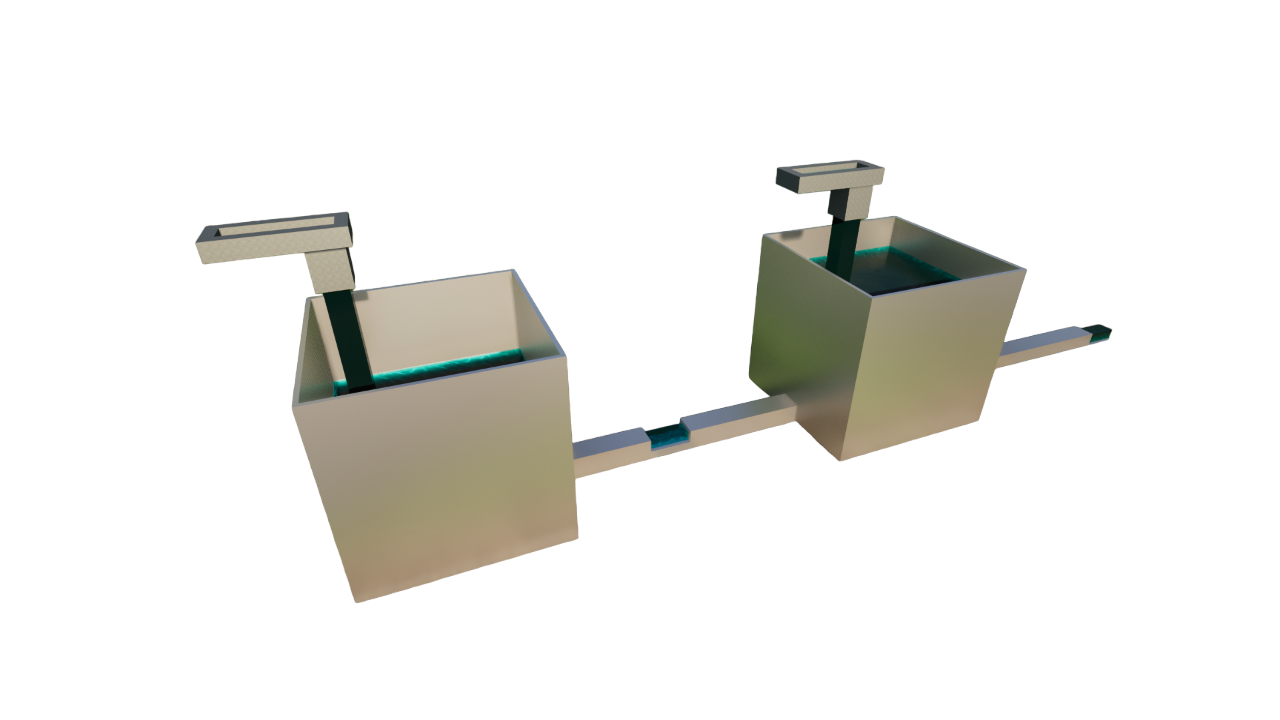
\includegraphics{/Users/follen/Desktop/SistemiDinamici/TESINA/assets/ritagliata.png}

\tableofcontents

\hypertarget{schema-del-sistema}{%
\subsection{Schema del sistema}\label{schema-del-sistema}}

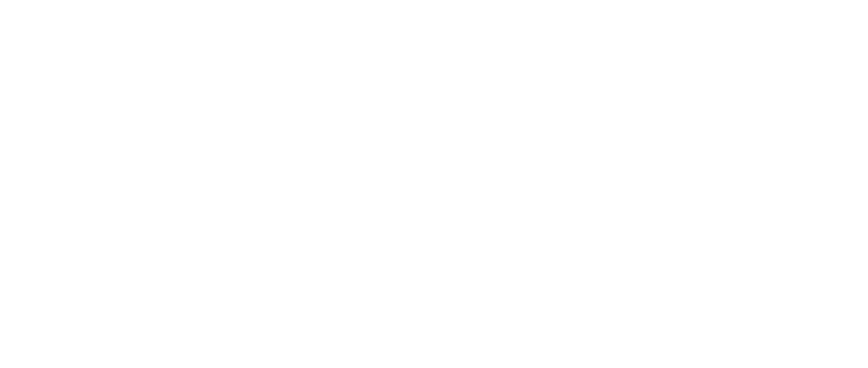
\includegraphics{/Users/follen/Desktop/SistemiDinamici/TESINA/assets/SchemaDarkModeNoBG.png}

\begin{quote}
Schema del sistema idraulico composto da due serbatoi.
\end{quote}

\hypertarget{circuito-equivalente}{%
\subsubsection{Circuito Equivalente}\label{circuito-equivalente}}

E` possibile rappresentare lo schema idraulico in termini di
\textbf{circuito elettrico}, con le componenti che conosciamo, andando a
sostituire:

\begin{longtable}[]{@{}ll@{}}
\toprule\noalign{}
Schema Idraulico & Schema Elettrico \\
\midrule\noalign{}
\endhead
\bottomrule\noalign{}
\endlastfoot
Serbatoio & Condensatore \\
Rubinetti & Generatori di corrente \\
Pressione atmosferica & Generatore di tensione \\
Resistenze idrauliche & Resistenze elettriche \\
Induttanze idrauliche & Induttanze idrauliche \\
\end{longtable}

Bisogna tenere a mente diversi accorgimenti:

\begin{itemize}
\item
  Come nello schema idraulico, le resistenze ed induttanze vanno poste
  tra due serbatoi (condensatori).
\item
  Tra un serbatoio e l\textquotesingle altro, se connessi, scorre un
  flusso qn; nello schema elettrico questo si traduce nel flusso,
  elettrico, ovvero in \emph{corrente elettrica}.
\end{itemize}

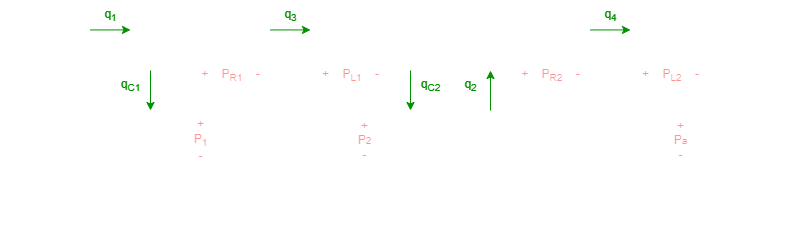
\includegraphics{/Users/follen/Desktop/SistemiDinamici/TESINA/assets/CircuitoEquivalenteRichDark.drawio.png}

\begin{quote}
Circuito equivalente
\end{quote}

\hypertarget{equazioni-del-sistema}{%
\subsubsection{Equazioni del sistema}\label{equazioni-del-sistema}}

A partire dal circuito equivalente è possibile estrapolare le equazioni
del sistema, che lo descrivono:

\begin{equation}
    \begin{cases}
      C_{1} \cdot \frac{\mathrm{d} }{\mathrm{d} t}P_{1} = q_{1} - q_{3}\\
      C_{2} \cdot \frac{\mathrm{d} }{\mathrm{d} t}P_{2} = q_{2} + q_{3} - q_{4}\\
      L_{1} \cdot \frac{\mathrm{d} }{\mathrm{d} t}q_{3} = -R_{1} \cdot q_{3} + p_{1} - p_{2}\\
      L_{2} \cdot \frac{\mathrm{d} }{\mathrm{d} t}q_{4} = -R_{1} \cdot q_{4} + p_{1} - p_{a}\\

    \end{cases}\,
\end{equation}

Ricordando la natura del sistema, possiamo identificare i valori di
input:

\begin{itemize}
\item
  \textbf{Input:}

  \begin{itemize}
  \item
    q1 : flusso in immissione tank 1
  \item
    q2 : flusso in immissione tank 2
  \item
    Pa: Pressione atmosferica "a valle"; Se si considera questa
    pressione molto più piccola rispetto alla pressione alla base del
    tank 2, la si può ignorare.
  \end{itemize}
\end{itemize}

\hypertarget{modello-nello-spazio-di-stato}{%
\subsubsection{Modello nello spazio di
stato}\label{modello-nello-spazio-di-stato}}

Possiamo quindi partire dalle equazioni del sistema e rappresentarlo
nello spazio di stato, andando a scegliere \textbf{Variabili di stato},
\textbf{Entrate} ed \textbf{uscite}:

\begin{equation}\\Variabili \ di \ stato
    \begin{cases}
x_{1} = P_{1}\\
x_{2} = P_{2}\\
x_{3} = q_{3}\\
    \end{cases}\
\end{equation}

\begin{equation}input
\begin{cases}
u_{1} = q_{1}\\
u_{2} = q_{2}\\
u_{3} = P_{a}\\
    \end{cases}\,
\end{equation}

\begin{equation}uscita
\begin{cases}
y_{1} = P_{1}\\
    \end{cases}\
\end{equation}

Possiamo scrivere sottoforma di matrice:


\includegraphics{/Users/follen/Desktop/SistemiDinamici/TESINA/assets/matrici_light_hq.png}

Possiamo inoltre "scegliere" l\textquotesingle uscita del sistema che
vogliamo monitorare, per questo esempio scegliamo la \emph{pressione
P1}, che per semplicità coincide proprio con la variabile di stato
\emph{x1}:


\includegraphics{/Users/follen/Desktop/SistemiDinamici/TESINA/assets/uscita_matrice.png}

\hypertarget{funzione-di-trasferimento-calcolata-con-matlab}{%
\paragraph{Funzione di trasferimento calcolata con
MatLab}\label{funzione-di-trasferimento-calcolata-con-matlab}}

Siccome la funzione di questo sistema risulta complicata da calcolare "a
mano", possiamo servirci di \textbf{MatLab}, che una volta immessi i
parametri del sistema tramite spazio di stato, può restituirci la
\textbf{Funzione Di Trasferimento} \emph{numerica} del sistema:

\hypertarget{immissione-delle-matrici}{%
\subparagraph{Immissione delle matrici}\label{immissione-delle-matrici}}

Dopo aver dichiarato i parametri, possiamo immettere le matrici appena
trovate all\textquotesingle interno dell\textquotesingle ambiente
MatLab; queste equazioni descrivono il sistema.

\begin{Shaded}
\begin{Highlighting}[]
\VariableTok{A} \OperatorTok{=}\NormalTok{ [   }\FloatTok{0}\OperatorTok{,}      \FloatTok{0}\OperatorTok{,}      \OperatorTok{{-}}\FloatTok{1}\OperatorTok{/}\VariableTok{C1}\OperatorTok{,}      \FloatTok{0}\OperatorTok{;}
        \FloatTok{0}\OperatorTok{,}      \FloatTok{0}\OperatorTok{,}      \FloatTok{1}\OperatorTok{/}\VariableTok{C2}\OperatorTok{,}       \OperatorTok{{-}}\FloatTok{1}\OperatorTok{/}\VariableTok{C2}\OperatorTok{;}
        \FloatTok{1}\OperatorTok{/}\VariableTok{L1}\OperatorTok{,}   \OperatorTok{{-}}\FloatTok{1}\OperatorTok{/}\VariableTok{L1}\OperatorTok{,}  \OperatorTok{{-}}\VariableTok{R1}\OperatorTok{/}\VariableTok{L1}\OperatorTok{,}      \FloatTok{0}\OperatorTok{;}
        \FloatTok{0}\OperatorTok{,}      \FloatTok{1}\OperatorTok{/}\VariableTok{L2}\OperatorTok{,}   \FloatTok{0}\OperatorTok{,}          \OperatorTok{{-}}\VariableTok{R2}\OperatorTok{/}\VariableTok{L2}
\NormalTok{    ]}\OperatorTok{;}

\VariableTok{B} \OperatorTok{=}\NormalTok{ [   }\FloatTok{1}\OperatorTok{/}\VariableTok{C1}\OperatorTok{,}   \FloatTok{0}\OperatorTok{,}      \FloatTok{0}\OperatorTok{;}
        \FloatTok{0}\OperatorTok{,}      \FloatTok{1}\OperatorTok{/}\VariableTok{C2}\OperatorTok{,}   \FloatTok{0}\OperatorTok{;}
        \FloatTok{0}\OperatorTok{,}      \FloatTok{0}\OperatorTok{,}      \FloatTok{0}\OperatorTok{;}
        \FloatTok{0}\OperatorTok{,}      \FloatTok{0}\OperatorTok{,}      \OperatorTok{{-}}\FloatTok{1}\OperatorTok{/}\VariableTok{L2}
\NormalTok{    ]}\OperatorTok{;}

\VariableTok{C} \OperatorTok{=}\NormalTok{ [}\FloatTok{1}\OperatorTok{,} \FloatTok{0}\OperatorTok{,} \FloatTok{0}\OperatorTok{,} \FloatTok{0}\NormalTok{]}\OperatorTok{;}
\VariableTok{D} \OperatorTok{=}\NormalTok{ [}\FloatTok{0}\OperatorTok{,} \FloatTok{0}\OperatorTok{,} \FloatTok{0}\NormalTok{]}\OperatorTok{;}
\end{Highlighting}
\end{Shaded}

\hypertarget{calcolo-della-funzione-di-trasferimento}{%
\subparagraph{Calcolo della funzione di
trasferimento}\label{calcolo-della-funzione-di-trasferimento}}

Con i seguenti comandi possiamo trovare \emph{\textbf{le}} funzioni di
trasferimento associate ai diversi input:

\begin{Shaded}
\begin{Highlighting}[]
\VariableTok{G} \OperatorTok{=} \VariableTok{ss}\NormalTok{(}\VariableTok{A}\OperatorTok{,} \VariableTok{B}\OperatorTok{,} \VariableTok{C}\OperatorTok{,} \VariableTok{D}\NormalTok{)}\OperatorTok{;}         \CommentTok{\% Sistema a partire dallo spazio di stato              }

\VariableTok{TFs} \OperatorTok{=} \VariableTok{tf}\NormalTok{(}\VariableTok{G}\NormalTok{)}\OperatorTok{;}                \CommentTok{\% Funzioni di trasferimento per i diversi input}
\end{Highlighting}
\end{Shaded}

Possiamo accedere ad una delle funzioni di trasferimento con il comando
\texttt{Tfs(k)}; viene di seguito riportato la FDT numerica associata
all\textquotesingle input 1:

\[G(s)_{1} = \frac{0,01s^3+0.02s^2+0.01s+16\cdot 10^{-4}}{s^4 + 2s^3 +1.03s^2+26\cdot10^{-2}+8.3\cdot10^{5}}\]

\hypertarget{risposta-del-sistema-nel-tempo}{%
\subsection{Risposta del sistema nel
tempo}\label{risposta-del-sistema-nel-tempo}}

Dopo aver rappresentato il sistema nell\textquotesingle ambiente MatLab,
possiamo iniziare ad ottenere informazioni sulle possibili risposte del
sistema.

La prima cosa che possiamo fare è controllare la posizione dei
\textbf{poli} e degli \textbf{zeri} nel piano complesso; questo è
possibile tramite il comando \texttt{pzmap(G)}, che restituisce il
seguente grafico:

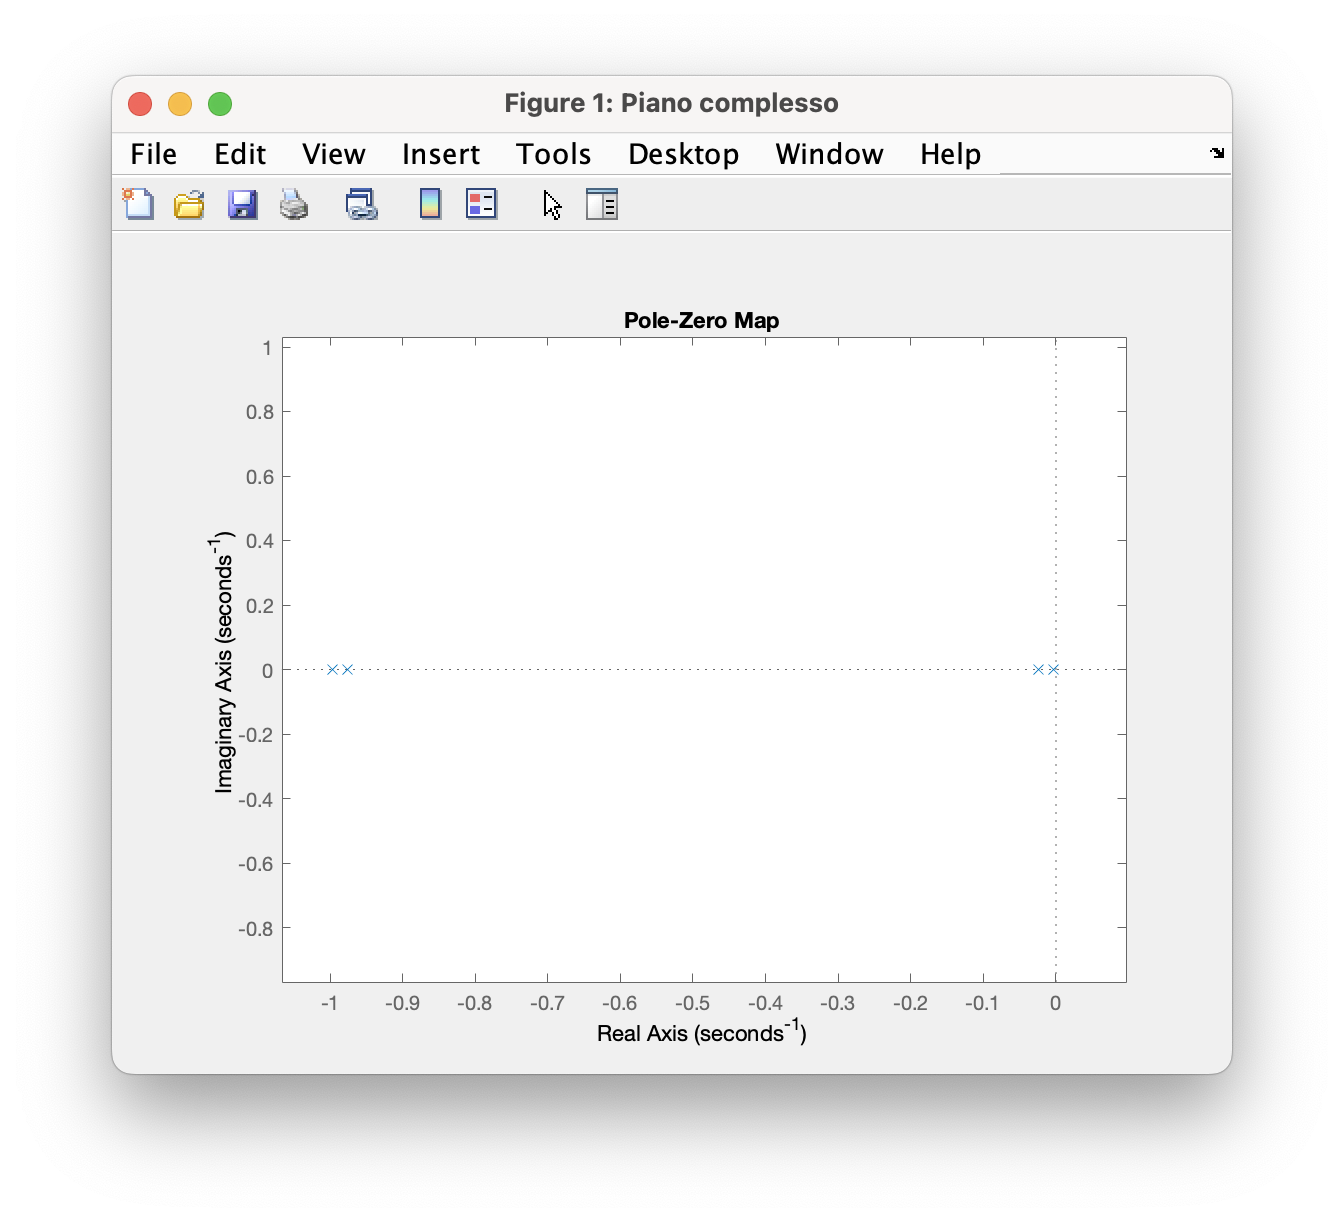
\includegraphics{/Users/follen/Desktop/SistemiDinamici/TESINA/assets/image-20240106112015562.png}

Dopo aver visualizzato i diversi poli e zeri del sistema, possiamo
passare a trovare l\textquotesingle uscita del sistema ad un segnale;
siccome il sistema è composto di 3 input, nel momento in cui calcoliamo
\texttt{step(G)}, ovvero la risposta ad un segnale gradino, matlab
"mette in ingresso" un gradino unitario \textbf{a tutti e 3 gli input}.

Capiamo quindi che questo modo è un po\textquotesingle{} troppo
limitante per il calcolo dell\textquotesingle uscita.

Possiamo però "costruirci" un segnale custom da utilizzare come uno (o
più) degli input del sistema; vediamo come fare:

\hypertarget{risposta-ad-un-segnale-custom}{%
\subsubsection{Risposta ad un segnale
custom}\label{risposta-ad-un-segnale-custom}}

La prima cosa da fare è sicuramente quella di costrire
l\textquotesingle input personalizzato; vogliamo realizzare un segnale
gradino che parte da un\textquotesingle ampiezza 1, e che varia di
ampiezza (arrivando a 2) dopo 500s:

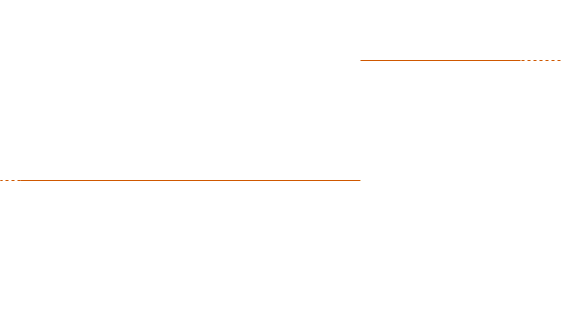
\includegraphics{/Users/follen/Desktop/SistemiDinamici/TESINA/assets/SegnaleDiIngresso.drawio.png}

Possiamo scrivere il segnale come somma di segnali elementari:

\begin{cases}
    u_{1}(t) = {\bf 1}(t) \\
    u_{2}(t) = {\bf 1}(t-500)
\end{cases}

\[u(t) = u_{1}(t) + u_{2}(t)\]

Possiamo trasformare il segnale nel dominio di Laplace ottenendo:

\begin{cases}
u_{1}(t) \longleftrightarrow U_{1}(s) = \frac{1}{s}\\
u_{2}(t) \longleftrightarrow U_{2}(s) = \frac{1}{s} \cdot e^{-100s}\\
\end{cases}

\[U(s) = U_{1}(s) + U_{2}(s)\]

Possiamo quindi costruire il segnale su MatLab "pezzo per pezzo" nel
seguente modo:

\begin{Shaded}
\begin{Highlighting}[]
\VariableTok{U21} \OperatorTok{=} \FloatTok{1}\OperatorTok{/}\VariableTok{s}\OperatorTok{;}                                  \CommentTok{\% Gradino unitario}
\VariableTok{U22} \OperatorTok{=} \VariableTok{tf}\NormalTok{([}\FloatTok{0} \FloatTok{1}\NormalTok{]}\OperatorTok{,}\NormalTok{ [}\FloatTok{1} \FloatTok{0}\NormalTok{]}\OperatorTok{,} \SpecialStringTok{\textquotesingle{}inputDelay\textquotesingle{}}\OperatorTok{,} \FloatTok{500}\NormalTok{)}\OperatorTok{;}  \CommentTok{\% Gradino ritardato di 100}
\VariableTok{U2} \OperatorTok{=} \VariableTok{U21} \OperatorTok{+} \VariableTok{U22}\OperatorTok{;}                             \CommentTok{\% Trovo il segnale risultante}
\end{Highlighting}
\end{Shaded}

Per trovare l\textquotesingle uscita ci basta quindi moltiplicare il
segnale (nel dominio di Laplace) per la funzione di trasferimento (che
abbiamo ottenuto tramite lo spazio di stato); bisogna stare attenti però
a "selezionare" la funzione di trasferimento giusta, perchè come abbiamo
già visto, le FDT sono 3, una per ogni input.

In questo caso vogliamo che il segnale sia attribuito
all\textquotesingle input 1, ovvero al flusso del tank 1, quindi
scegliamo la FDT 1:

\begin{Shaded}
\begin{Highlighting}[]
\VariableTok{Y3} \OperatorTok{=} \VariableTok{G\_default}\NormalTok{(}\FloatTok{1}\NormalTok{) }\OperatorTok{*} \VariableTok{U2}\OperatorTok{;}						\CommentTok{\% Calcolo l\textquotesingle{}uscita nel dominio di Laplace}
\NormalTok{[}\VariableTok{y2}\OperatorTok{,} \VariableTok{t2}\NormalTok{] }\OperatorTok{=} \VariableTok{impulse}\NormalTok{(}\VariableTok{Y3}\NormalTok{)}\OperatorTok{;}						\CommentTok{\% Calcolo l\textquotesingle{}antitrasformata}
\end{Highlighting}
\end{Shaded}

Possiamo calcolare l\textquotesingle antitrasformta con
\texttt{impulse(Y3)}, perché nel dominio di Laplace
l\textquotesingle impulso corrisponde ad \texttt{1}, quindi
moltiplicando per 1 il segnale \emph{Y(s)} non cambia; successivamente
provvede MatLab ad \emph{antri trasformare} (sempre con impulse).

\hypertarget{plot-dei-singoli-modi}{%
\subsubsection{Plot dei singoli modi}\label{plot-dei-singoli-modi}}

Possiamo quindi effettuare il plot dei singoli modi e dei segnali
totali:

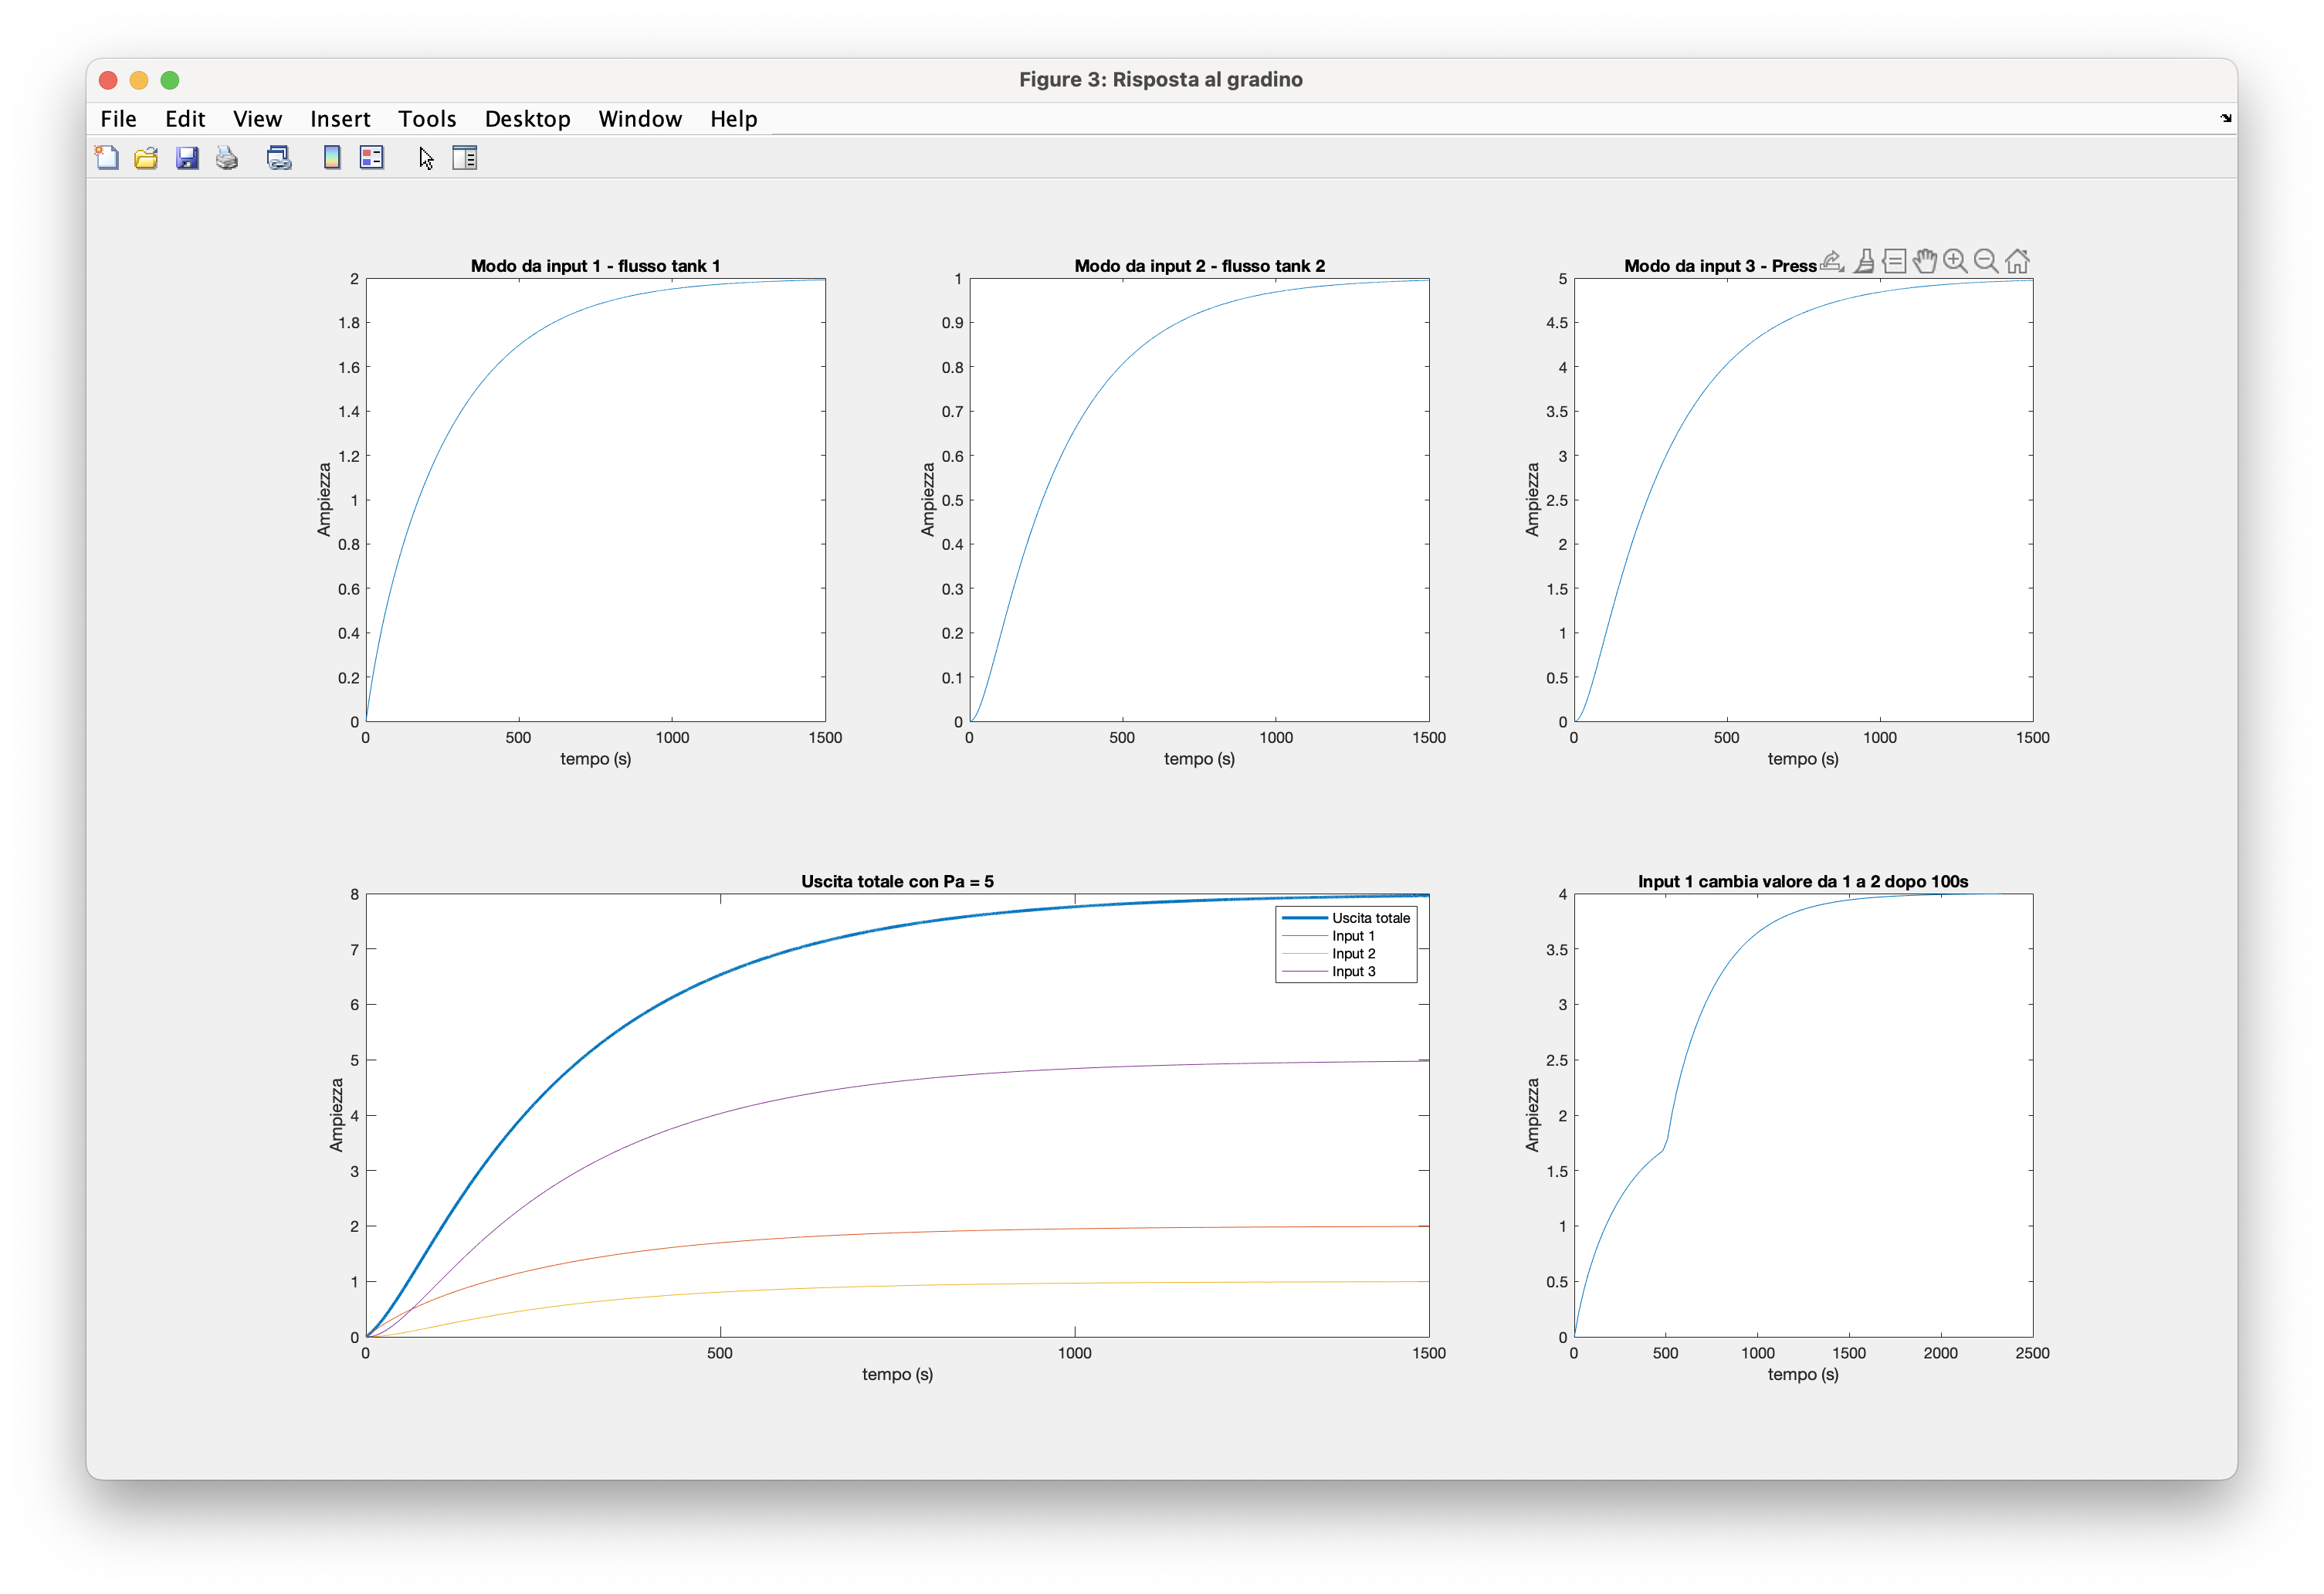
\includegraphics{/Users/follen/Desktop/SistemiDinamici/TESINA/assets/image-20240106113047528.png}

\begin{quote}
\begin{itemize}
\item
  \textbf{Plot 1}: modo dall\textquotesingle input 1 gradino unitario
  (q1)
\item
  Plot 2: modo dall\textquotesingle input 2 gradino unitario (q2)
\item
  Plot 3: modo dall\textquotesingle input 3 gradino di ampiezza 5 (Pa)
\item
  Plot 4:

  \begin{itemize}
  \item
    In Blu: uscita totale dei segnali 1, 2 e 3.
  \item
    Il resto dei plot sono i singoli modi.
  \end{itemize}
\item
  Plot 5: uscita totale agli input:

  \begin{itemize}
  \item
    in 1: gradino che inizia unitario e cambia valore in t=500 arrivando
    ad un valore pari a 2.
  \item
    in 2: gradino unitario.
  \item
    in 3: gradino unitario.
  \end{itemize}
\end{itemize}
\end{quote}

\hypertarget{risposta-del-sistema-al-variare-dei-parametri}{%
\subsubsection{Risposta del sistema al variare dei
parametri}\label{risposta-del-sistema-al-variare-dei-parametri}}

\hypertarget{risposta-al-variare-della-capacituxe0}{%
\paragraph{Risposta al variare della
capacità}\label{risposta-al-variare-della-capacituxe0}}

In questo esempio facciamo variare la capacità del tank 1, con il
seguente codice:

\begin{Shaded}
\begin{Highlighting}[]
\KeywordTok{for} \VariableTok{i}\OperatorTok{=}\FloatTok{1}\OperatorTok{:}\VariableTok{n}
    \VariableTok{G\_capcity\_1} \OperatorTok{=} \VariableTok{ss}\NormalTok{(}\VariableTok{A}\OperatorTok{,} \VariableTok{B}\OperatorTok{,} \VariableTok{C}\OperatorTok{,} \VariableTok{D}\NormalTok{)}\OperatorTok{;}       \CommentTok{\% Rappresento il sistema con il valore di C1 corrente}

\NormalTok{    [}\VariableTok{yn}\OperatorTok{,} \VariableTok{tn}\NormalTok{] }\OperatorTok{=} \VariableTok{step}\NormalTok{(}\VariableTok{G\_capcity\_1}\NormalTok{)}\OperatorTok{;}       \CommentTok{\% Calcolo la risposta al gradino unitario}
    \VariableTok{yn\_sum} \OperatorTok{=} \VariableTok{sum}\NormalTok{(}\VariableTok{yn}\OperatorTok{,}\NormalTok{ [}\FloatTok{2} \FloatTok{3}\NormalTok{])}\OperatorTok{;}            \CommentTok{\% Sommo le uscite dei 3 ingressi}
    \VariableTok{plot}\NormalTok{(}\VariableTok{tn}\OperatorTok{,} \VariableTok{yn\_sum}\NormalTok{)                    }\CommentTok{\% Disegno le diverse uscite}
    \VariableTok{hold} \VariableTok{on}\OperatorTok{;}

    \VariableTok{C1} \OperatorTok{=} \VariableTok{C1} \OperatorTok{+} \FloatTok{50}\OperatorTok{;}                       \CommentTok{\% Aggiorno il valore di C per la prossima iterazione}
\NormalTok{    [}\VariableTok{A}\OperatorTok{,} \VariableTok{B}\OperatorTok{,} \VariableTok{C}\OperatorTok{,} \VariableTok{D}\NormalTok{] }\OperatorTok{=} \VariableTok{updateMatrixes}\NormalTok{(}\VariableTok{C1}\OperatorTok{,} \VariableTok{C2}\OperatorTok{,} \VariableTok{R1}\OperatorTok{,} \VariableTok{R2}\OperatorTok{,} \VariableTok{L1}\OperatorTok{,} \VariableTok{L2}\NormalTok{)}\OperatorTok{;}  \CommentTok{\% Aggiorno le matrici con il valore di C corrente}
    \VariableTok{legend\_text}\NormalTok{\{}\VariableTok{i}\NormalTok{\} }\OperatorTok{=} \VariableTok{sprintf}\NormalTok{(}\StringTok{"Capacita\textquotesingle{} = \%i"}\OperatorTok{,} \VariableTok{C1}\NormalTok{)}\OperatorTok{;}         \CommentTok{\% Attribuisco ad ogni curva un nome per la legenda}
\KeywordTok{end}
\end{Highlighting}
\end{Shaded}

Andiamo quindi, ad ogni iterazione, ad aumentare la capacità del
serbatoio; possiamo notare dalle curve, che man mano che la capacità
aumenta, la pressione del sistema impiega sempre più tempo ad arrivare a
regime.

Notiamo, però, che il \emph{valore} di regime resta invariato.

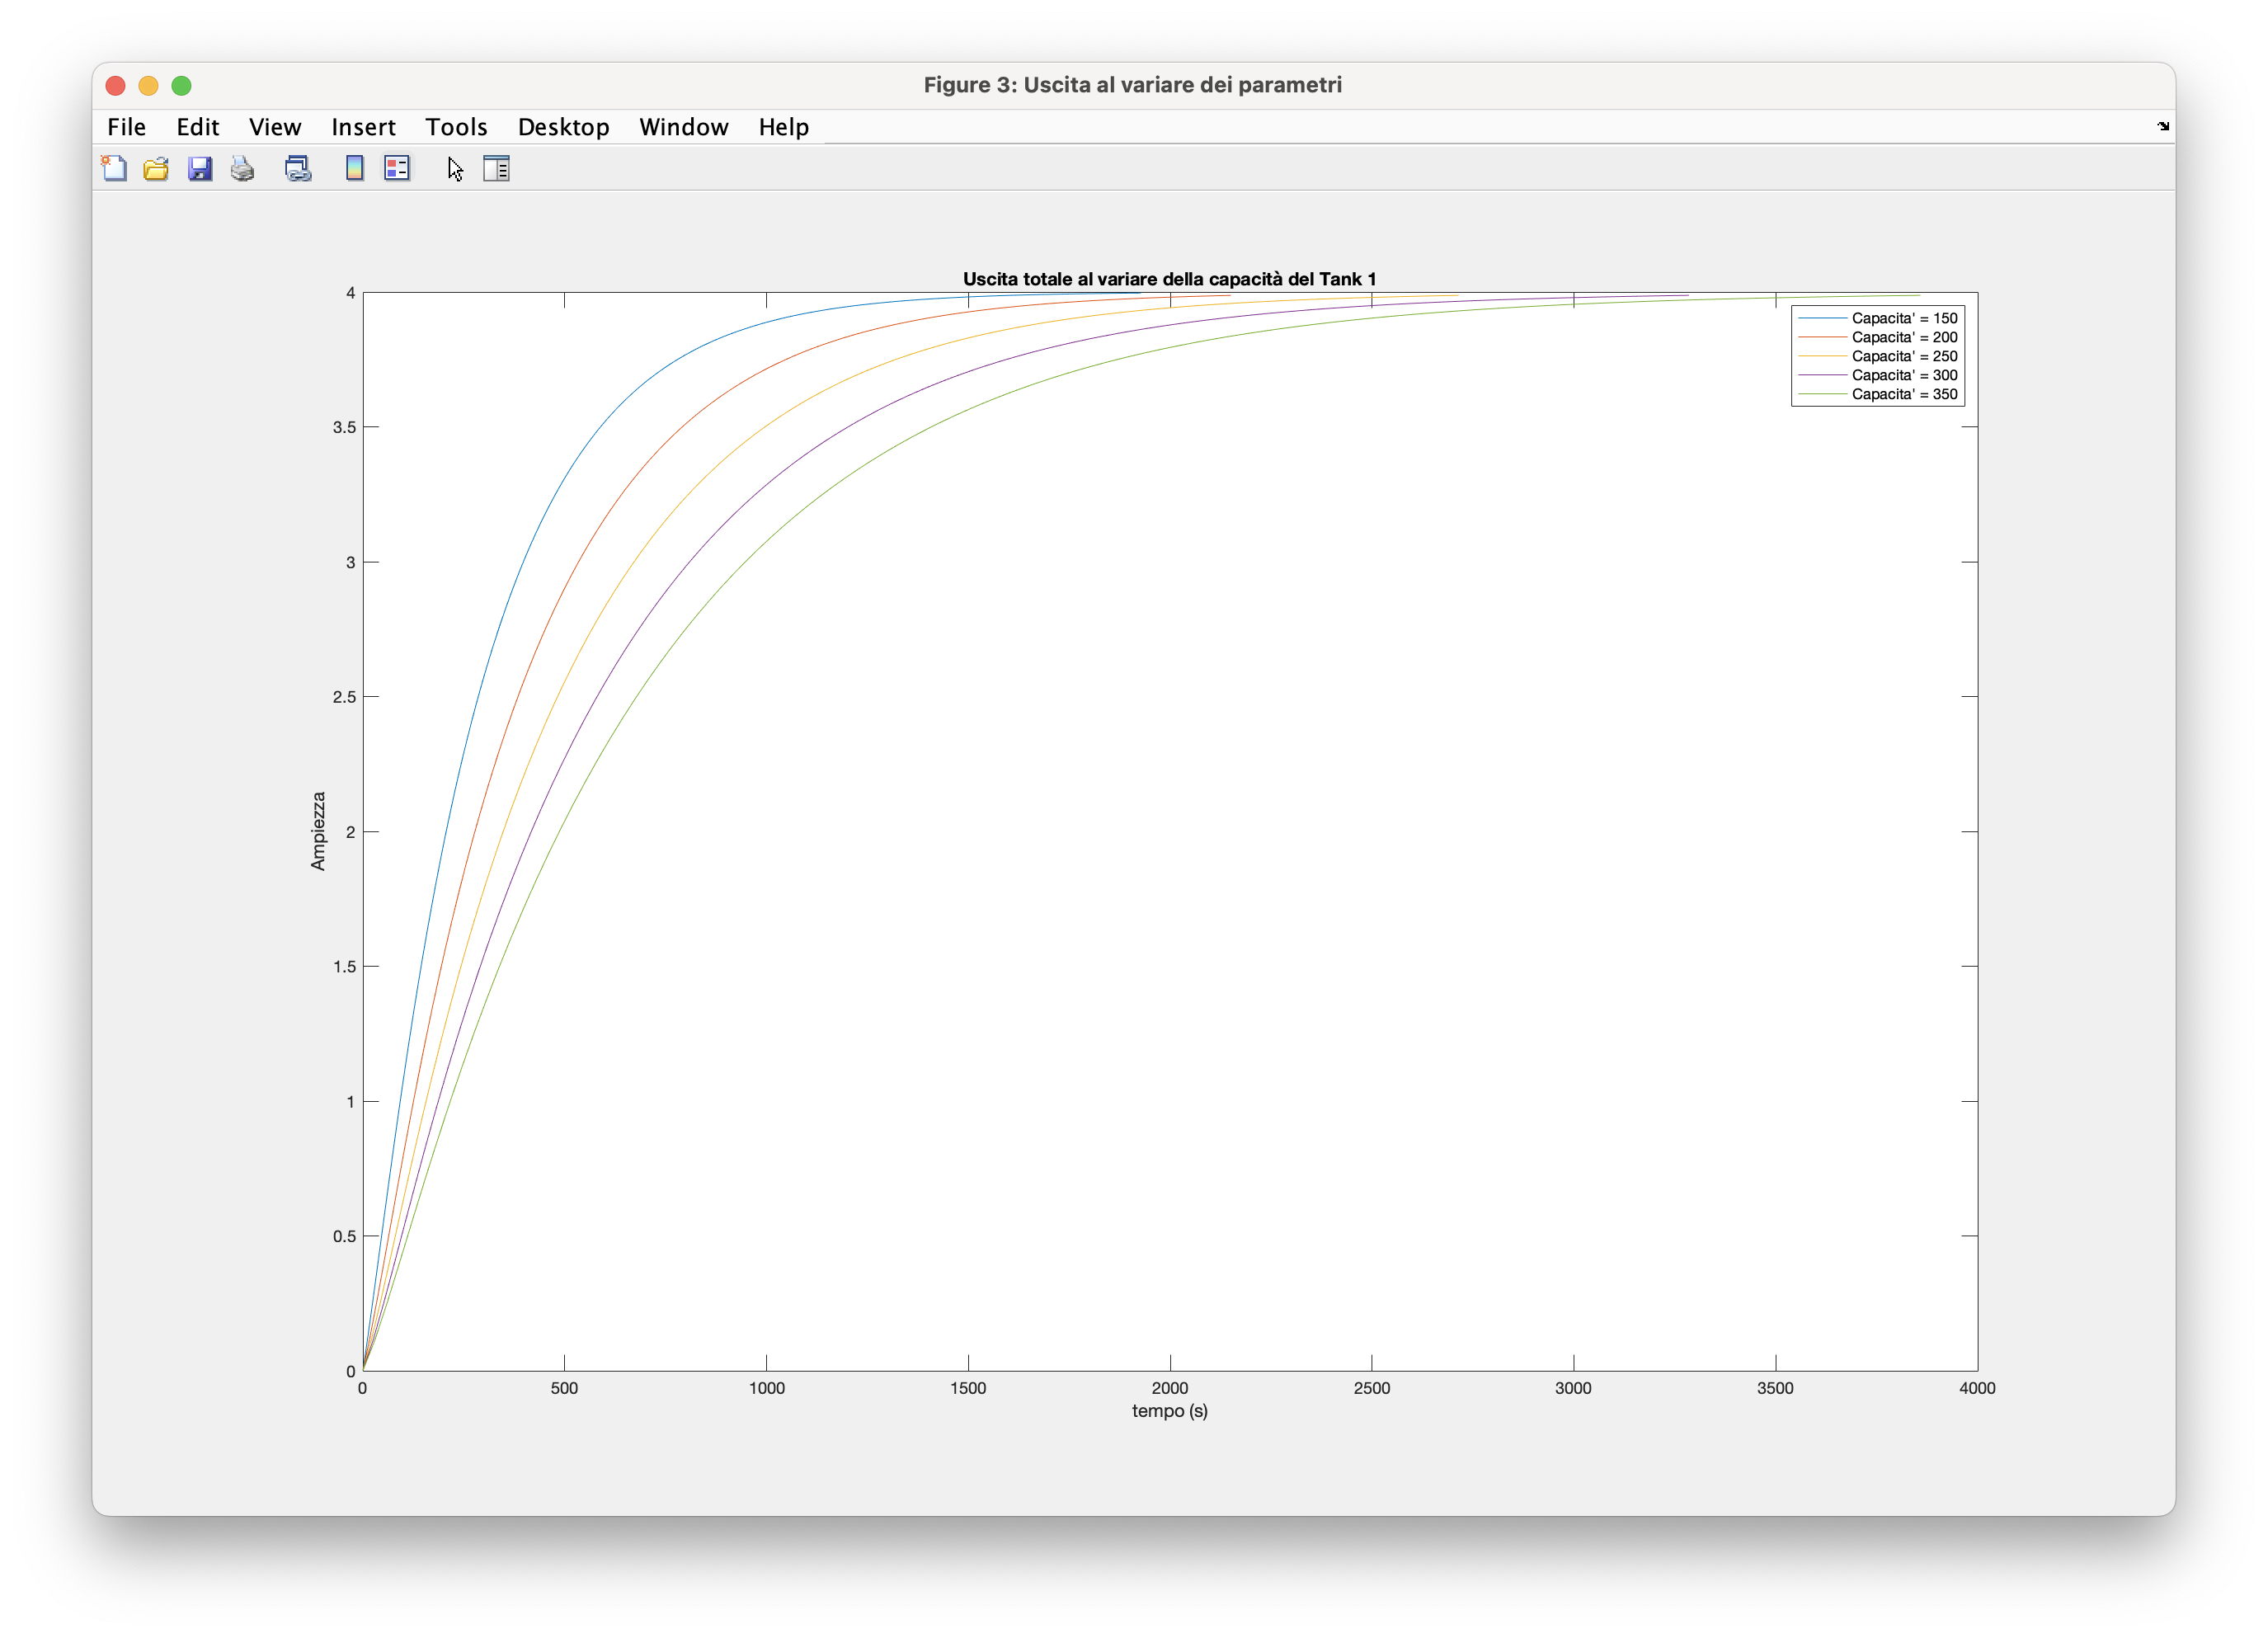
\includegraphics{/Users/follen/Desktop/SistemiDinamici/TESINA/assets/image-20240106113124504.png}

\hypertarget{risposta-al-variare-dellinduttanza}{%
\paragraph{Risposta al variare
dell\textquotesingle induttanza}\label{risposta-al-variare-dellinduttanza}}

Allo stesso modo possiamo far variare l\textquotesingle induttanza; ad
ogni iterazione variamo di un valore maggiore, in modo da ottenere un
risultato più "interessante":

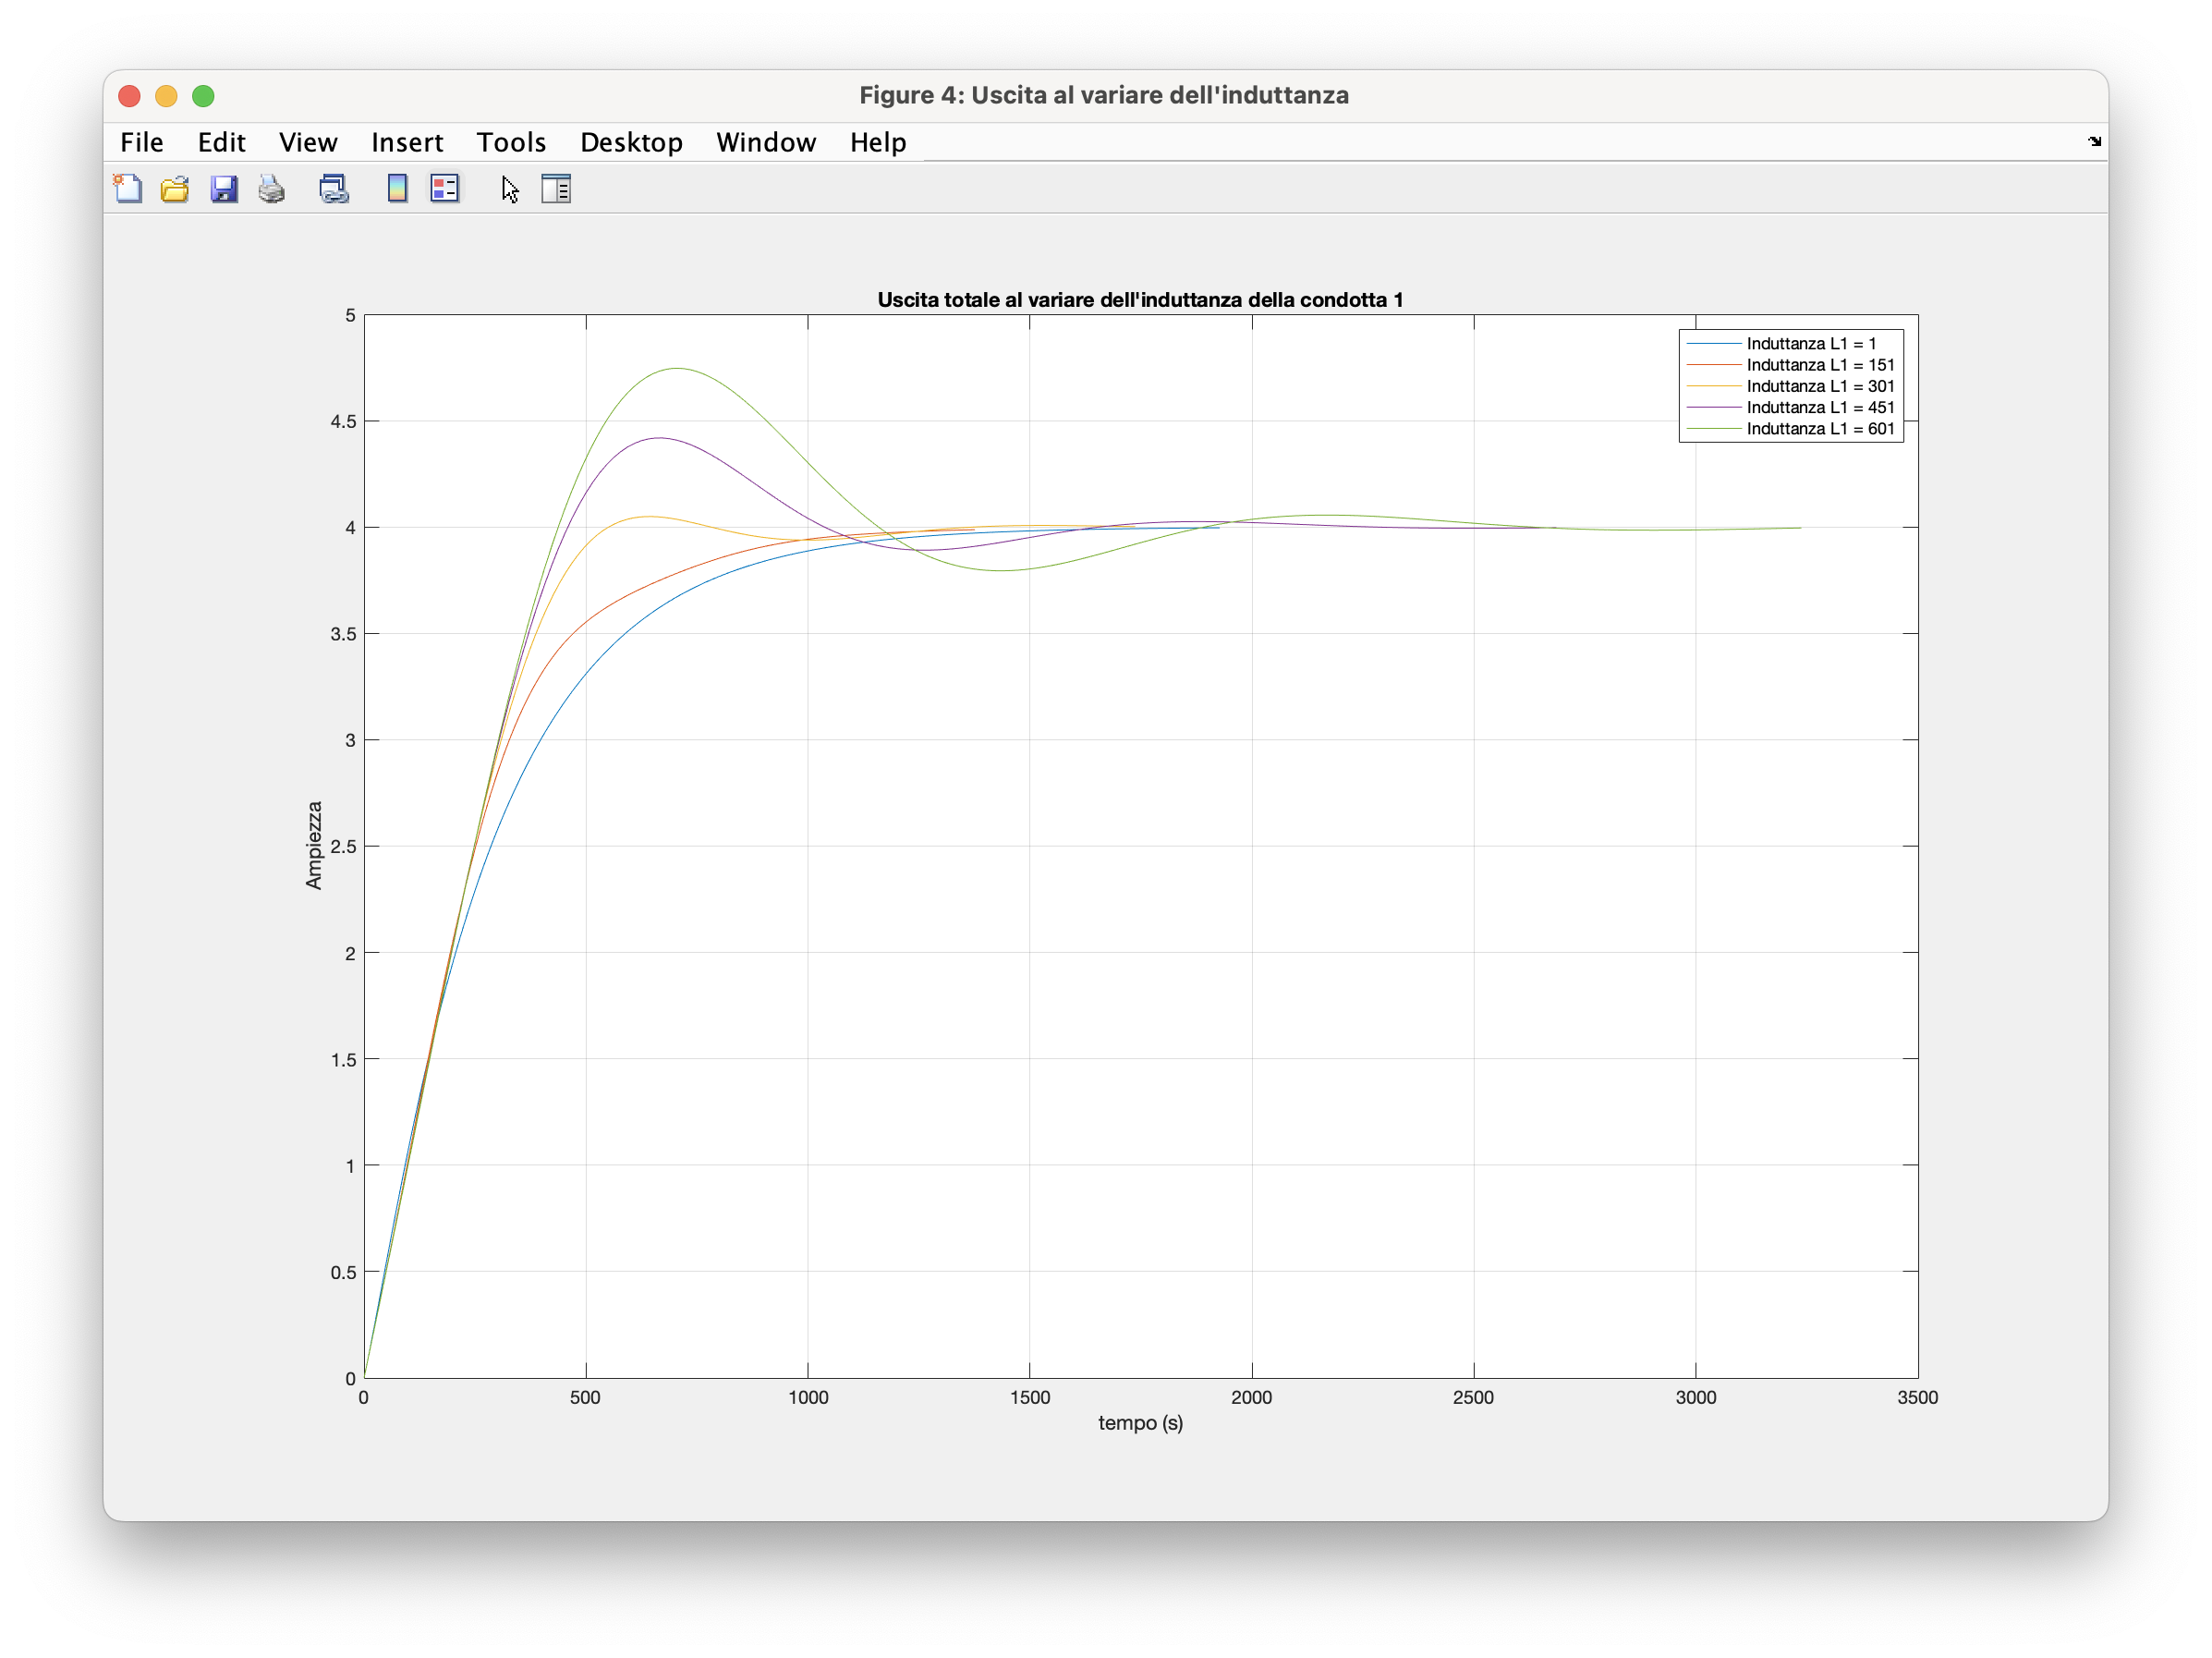
\includegraphics{/Users/follen/Desktop/SistemiDinamici/TESINA/assets/image-20240107210446106.png}

\hypertarget{risposta-al-variare-della-resistenza}{%
\paragraph{Risposta al variare della
resistenza}\label{risposta-al-variare-della-resistenza}}

Se la resistenza della condotta 1 aumenta, allora la pressione sul tank
1 aumenta, perchè il liquido avrà maggiore difficoltà a spostarsi dal
tank 1 al tank 2, infatti:

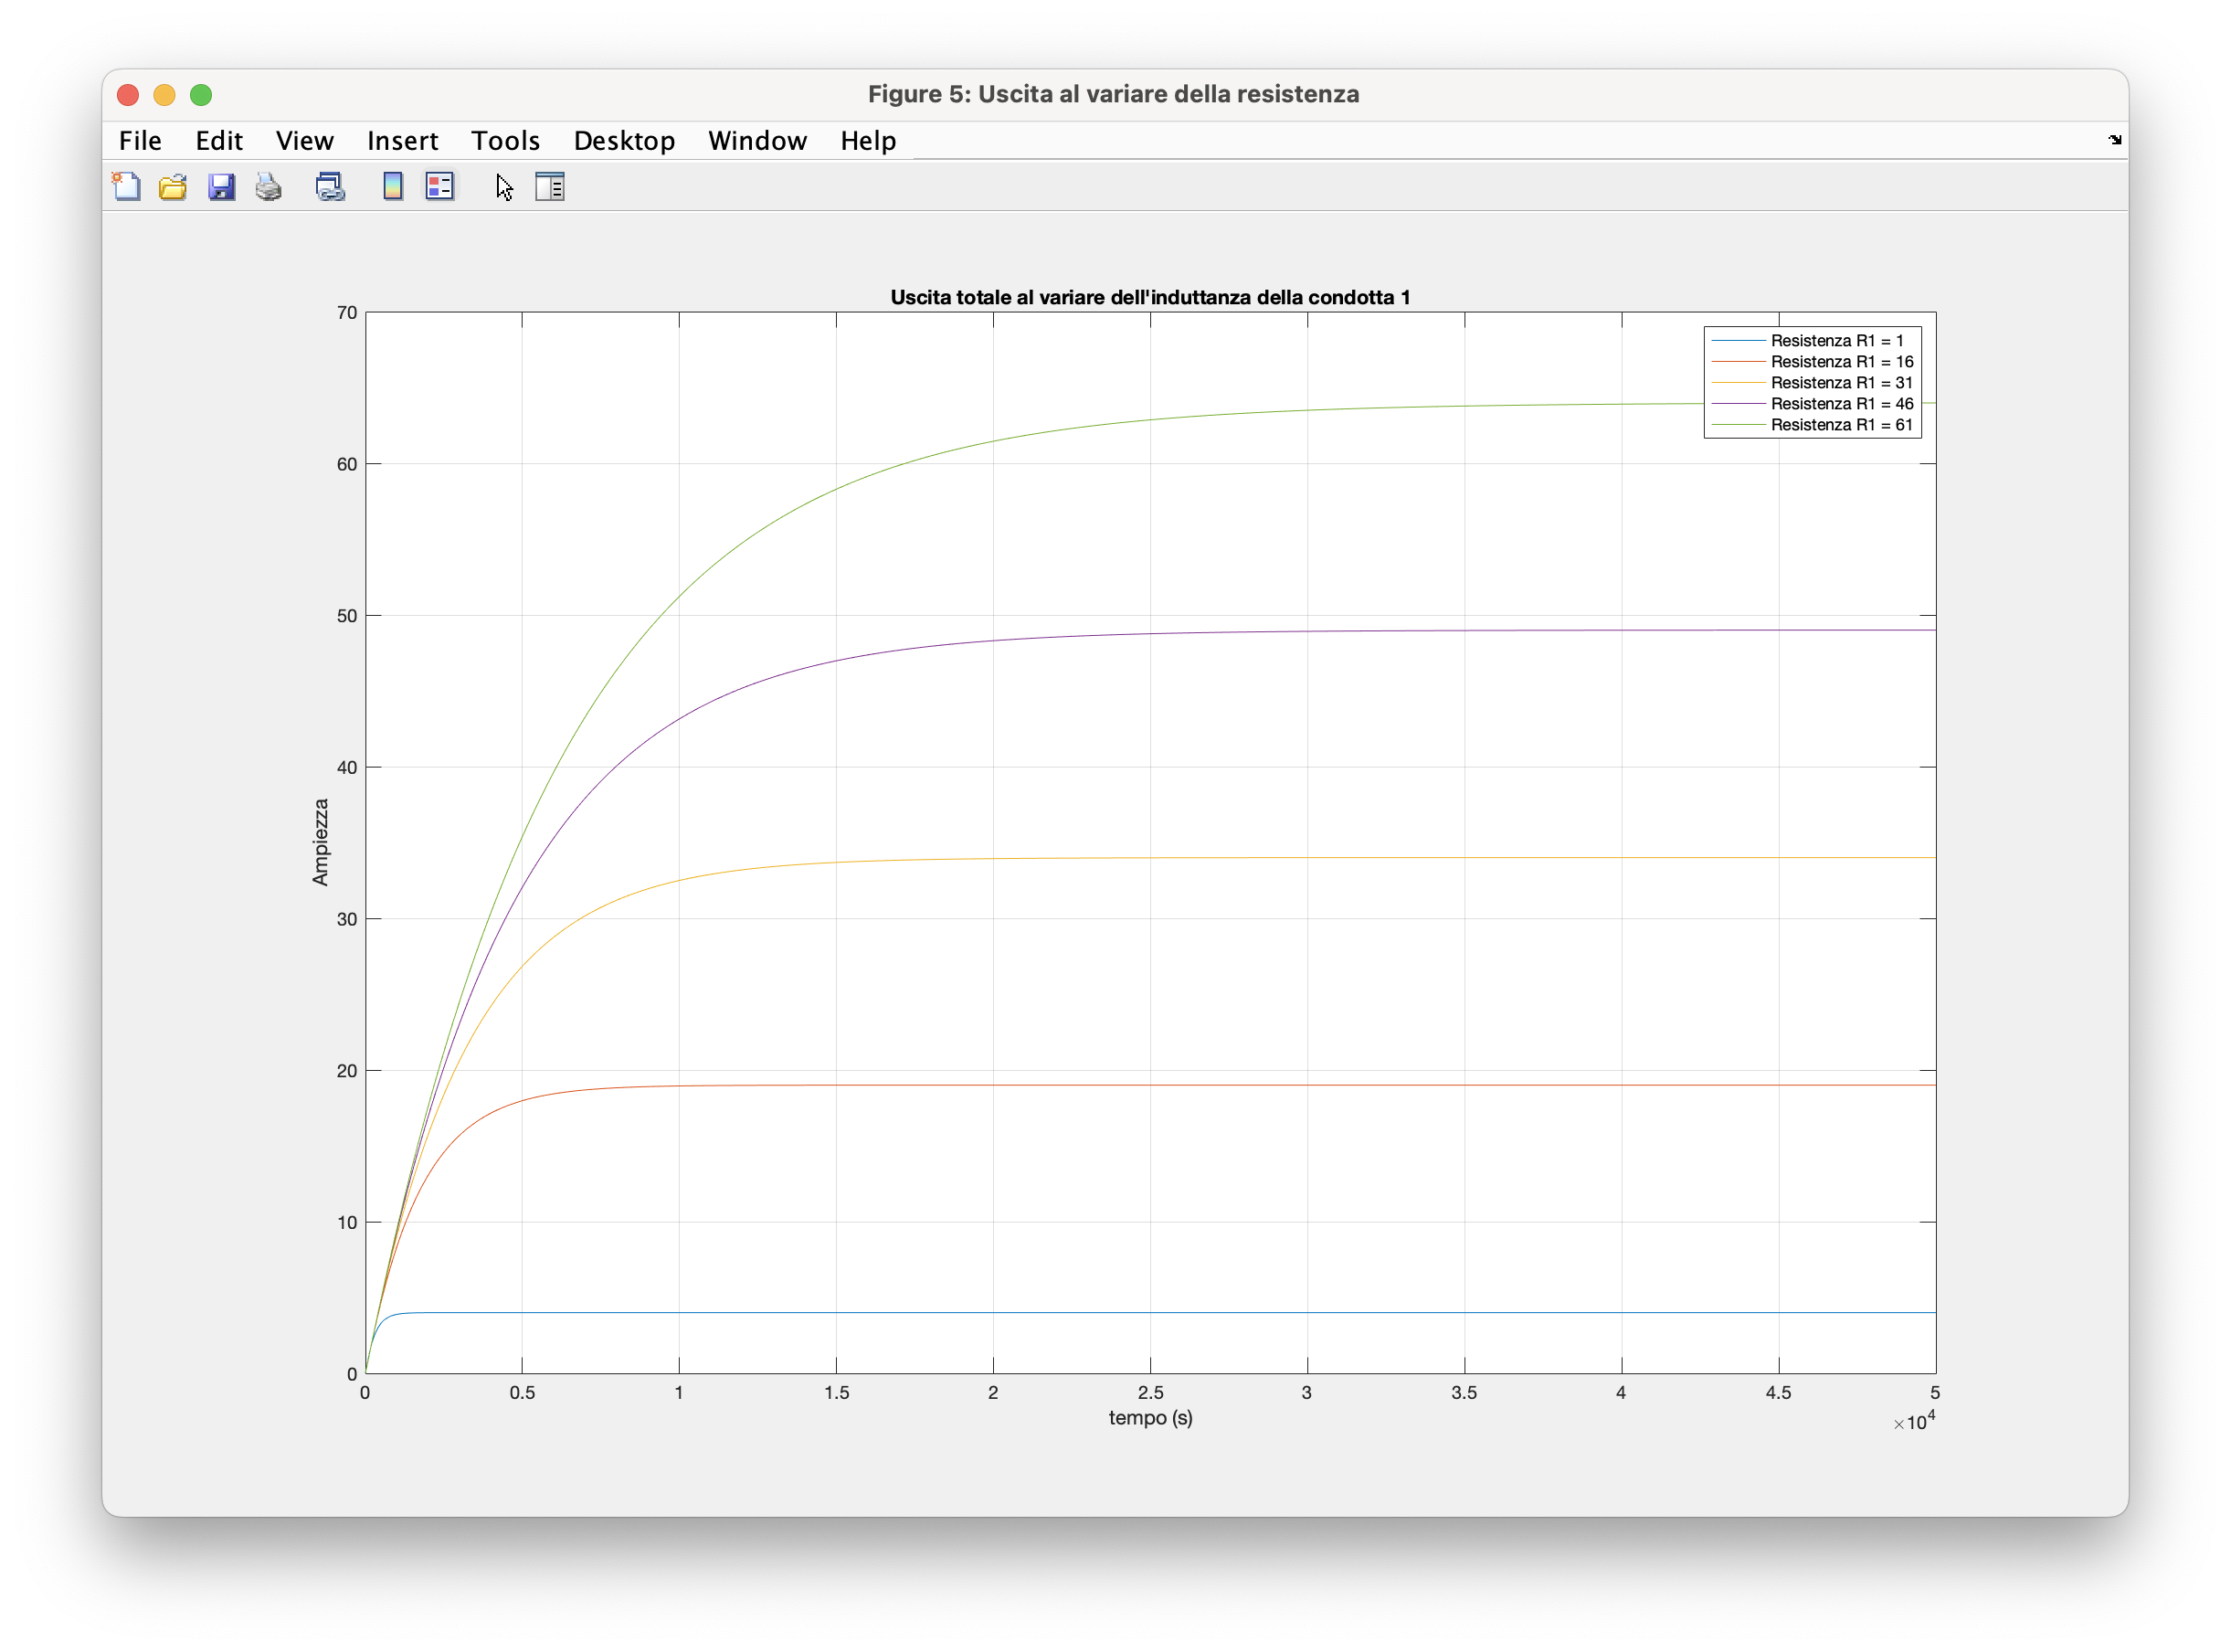
\includegraphics{/Users/follen/Desktop/SistemiDinamici/TESINA/assets/image-20240107210512401.png}

\hypertarget{diagrammi-di-bode}{%
\subsection{Diagrammi di Bode}\label{diagrammi-di-bode}}

Possiamo effettuare un\textquotesingle analisi anche dal punto di vista
della frequenza, andando a tracciare i \textbf{diagrammi di Bode}, sia
dei moduli che delle fasi:

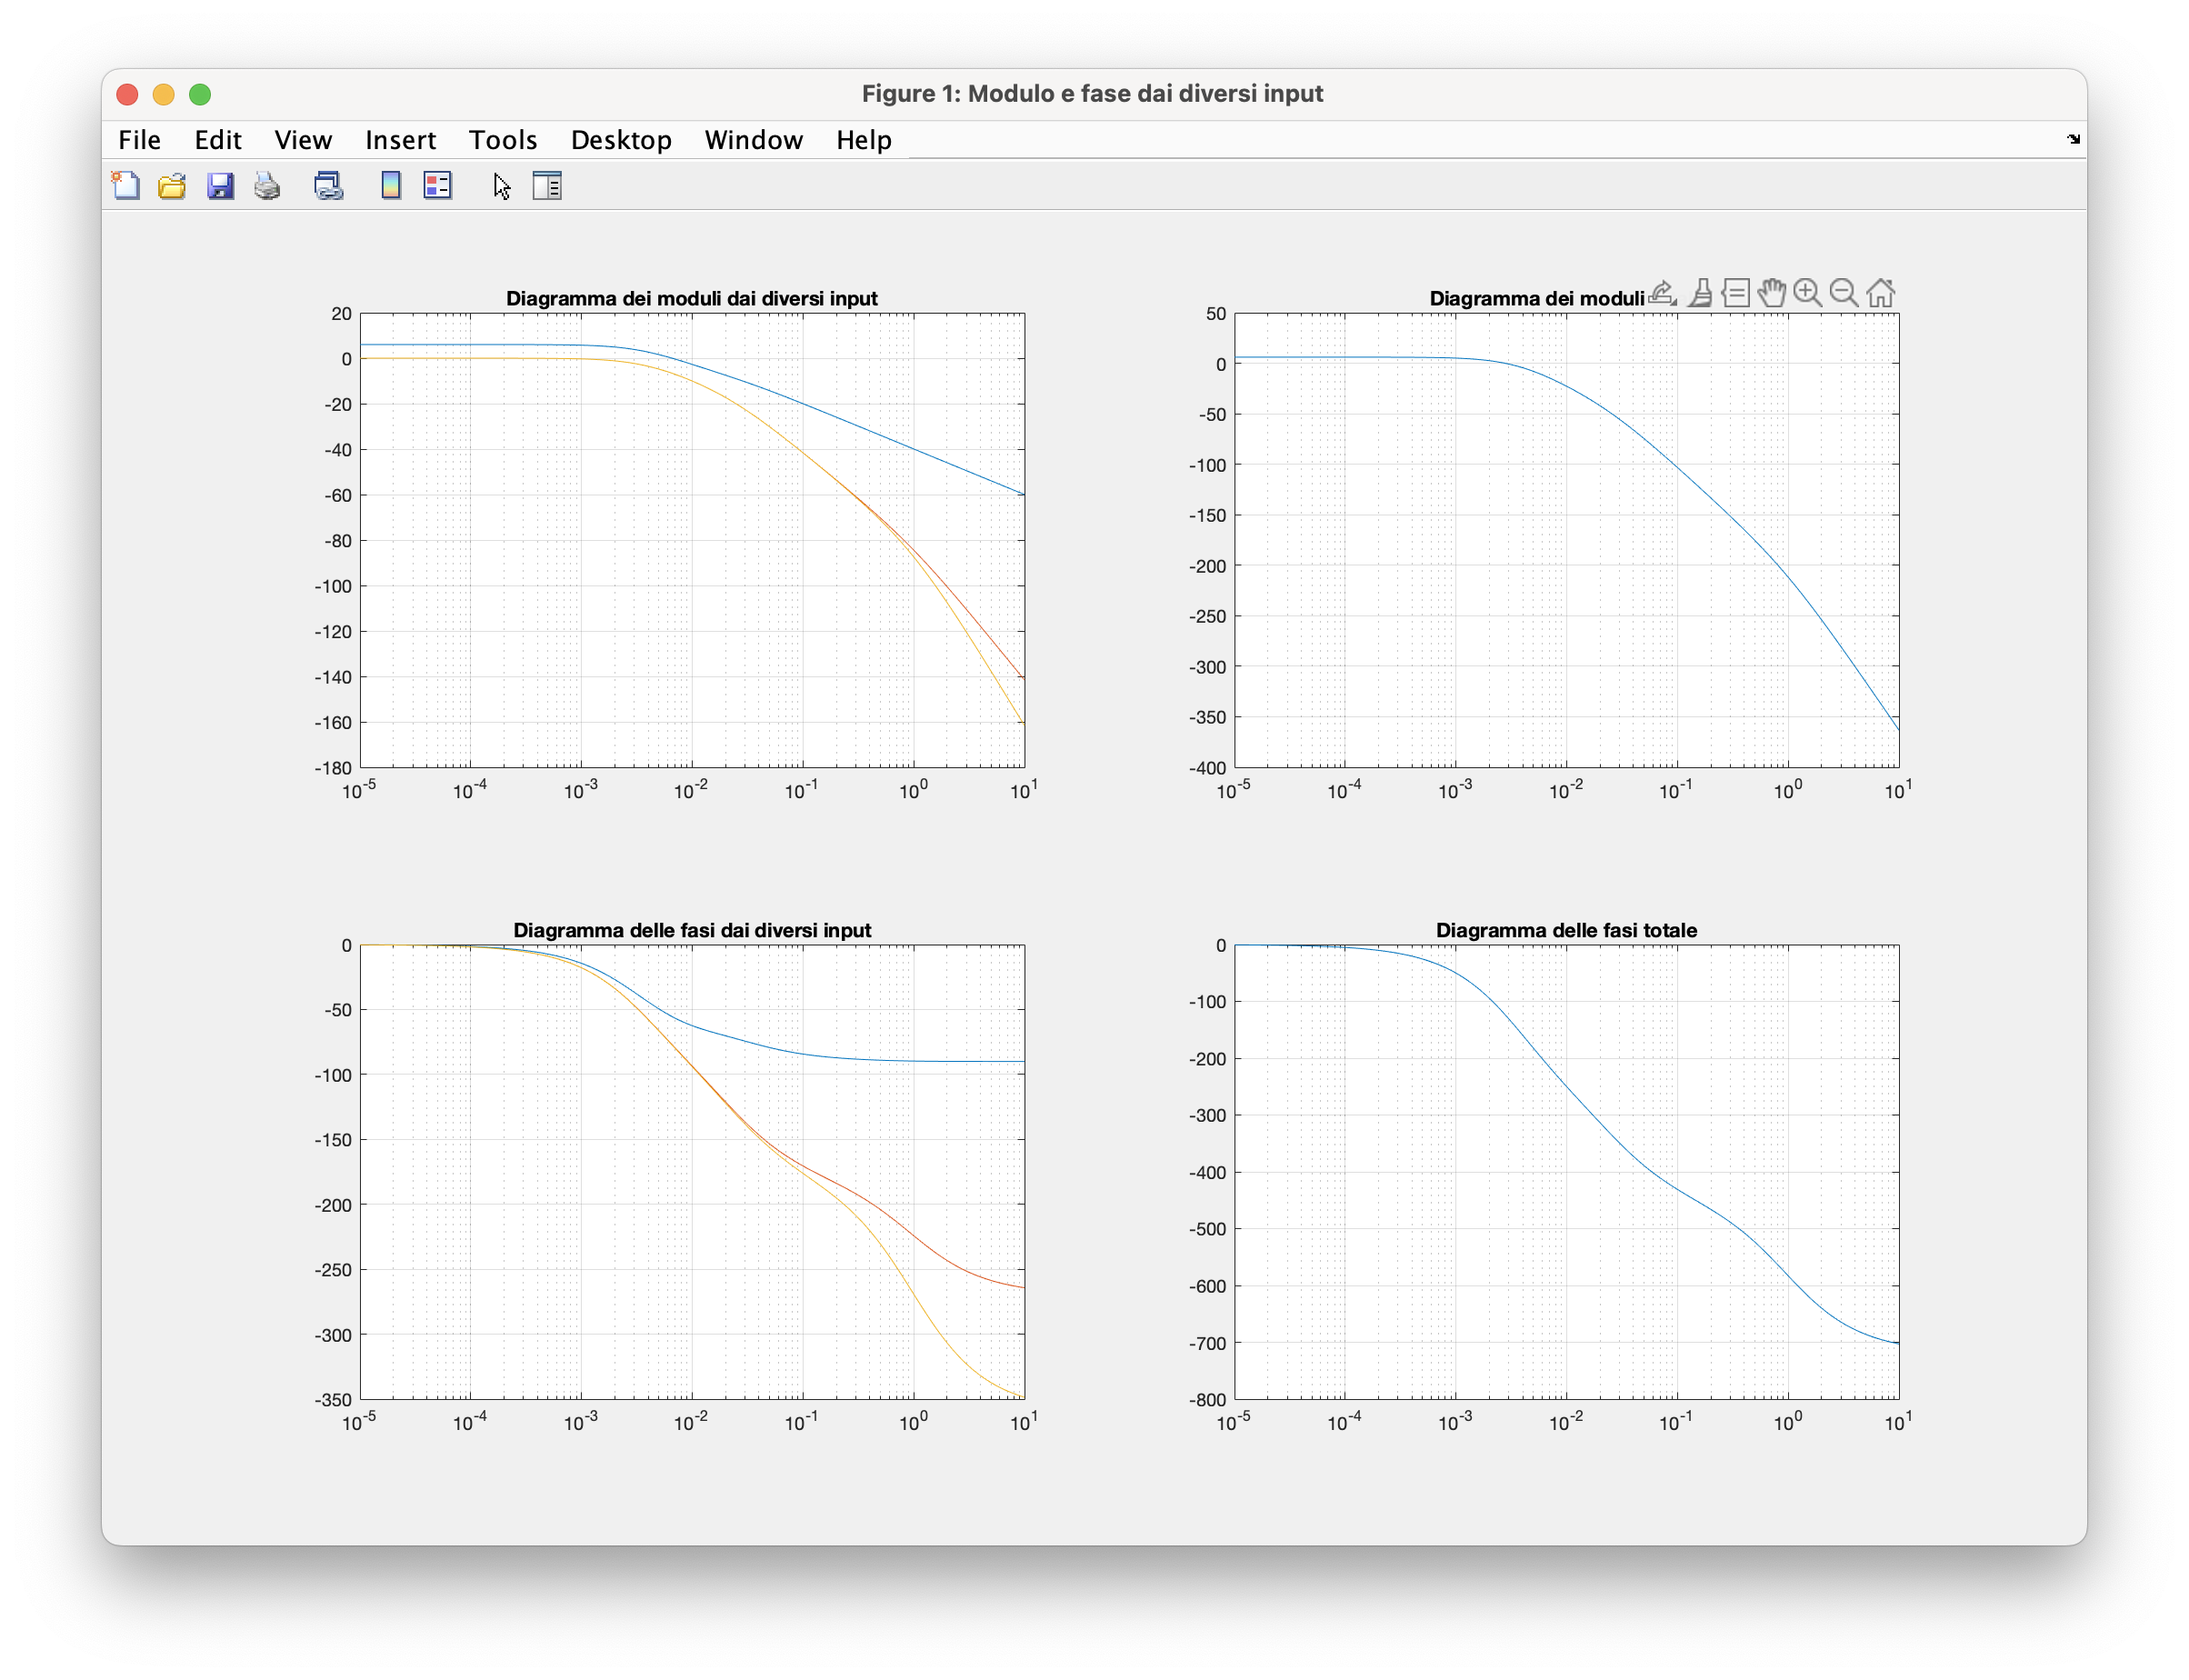
\includegraphics{/Users/follen/Desktop/SistemiDinamici/TESINA/assets/image-20240107211127030.png}

I diagrammi di Bode sono in grado di darci molte informazioni sul
sistema in esame; possiamo ad esempio vedere che tutte le frequenze
inferiori alla frequenza

\[\omega < 10^{-3} \ \ \ rad/s\]

vengono leggermente amplificate, mentre a partire da questa frequenza in
poi verranno attenuate.

\textbf{Ma cosa vuol dire?}

Essenzialmente stiamo dicendo che, data una sinusoide di una certa
ampiezza in ingresso del tipo:

\[u(t) = X \cdot sin(\omega_{0} \cdot t)\]

avremo in output un segnale sempre sinusoidale, ma con modulo e fase
cambiati, a seconda dei valori letti sui diagrammi di Bode:

\[y(t) = X \cdot |G(j\omega_{0})|_{dB} \ \cdot sin(\omega_{0} \cdot t \ + \angle{G(j\omega_{0})})\]

\hypertarget{lettura-del-diagramma-dei-moduli}{%
\subsubsection{Lettura del diagramma dei
moduli}\label{lettura-del-diagramma-dei-moduli}}

Di conseguenza, se sul diagramma dei moduli vedremo un valore positivo
(in corrispondenza della frequenza dell\textquotesingle ingresso u(t)),
sapremo che l\textquotesingle input verrà amplificato, mentre se vedremo
un valore negativo l\textquotesingle input verrà attenuato.

Otteniamo questo comportamento per via del fatto che sul diagramma di
Bode, i moduli vengono espressi in \textbf{deciBel}; un valore x0 può
essere convertito in deciBel secondo la formula:

\[x_{dB} = 20 \cdot log_{10}(x_{0})\]

Quindi, quando leggiamo il valore sul diagramma dei moduli, e lo
convertiamo nuovamente in valore naturale, seguendo la formula:

\[x_{dB} = 20 \cdot log_{10}(x_{0}) \Longrightarrow \ x_{0} = 10^{\frac{x_{dB}}{20}}\]

\hypertarget{lettura-del-diagramma-delle-fasi}{%
\subsubsection{Lettura del diagramma delle
fasi}\label{lettura-del-diagramma-delle-fasi}}

Il diagramma delle fasi ci dice se la fase della sinusoide in uscita è
\textbf{in anticipo o in ritardo} rispetto alla sinusoide in entrata; se
leggiamo, ad esempio, un valore di \emph{+90°}, questo vorrà dire che la
sinusoide in uscita è in anticipo di 90° rispetto al segnale in entrata.

Il segnale in uscita può anche essere \textbf{in fase} col segnale in
entrata, ovvero se, in corrispondenza di quella determinata frequenza,
il diagramma delle fasi riporta come valore \texttt{0}.

\hypertarget{uscita-steady-state}{%
\subsubsection{Uscita "Steady State"}\label{uscita-steady-state}}

Possiamo quindi trovare l\textquotesingle uscita \textbf{Steady State},
ovvero la risposta del sistema dopo che il \emph{transitorio} si è
esaurito, e l\textquotesingle uscita \textbf{è a regime}.

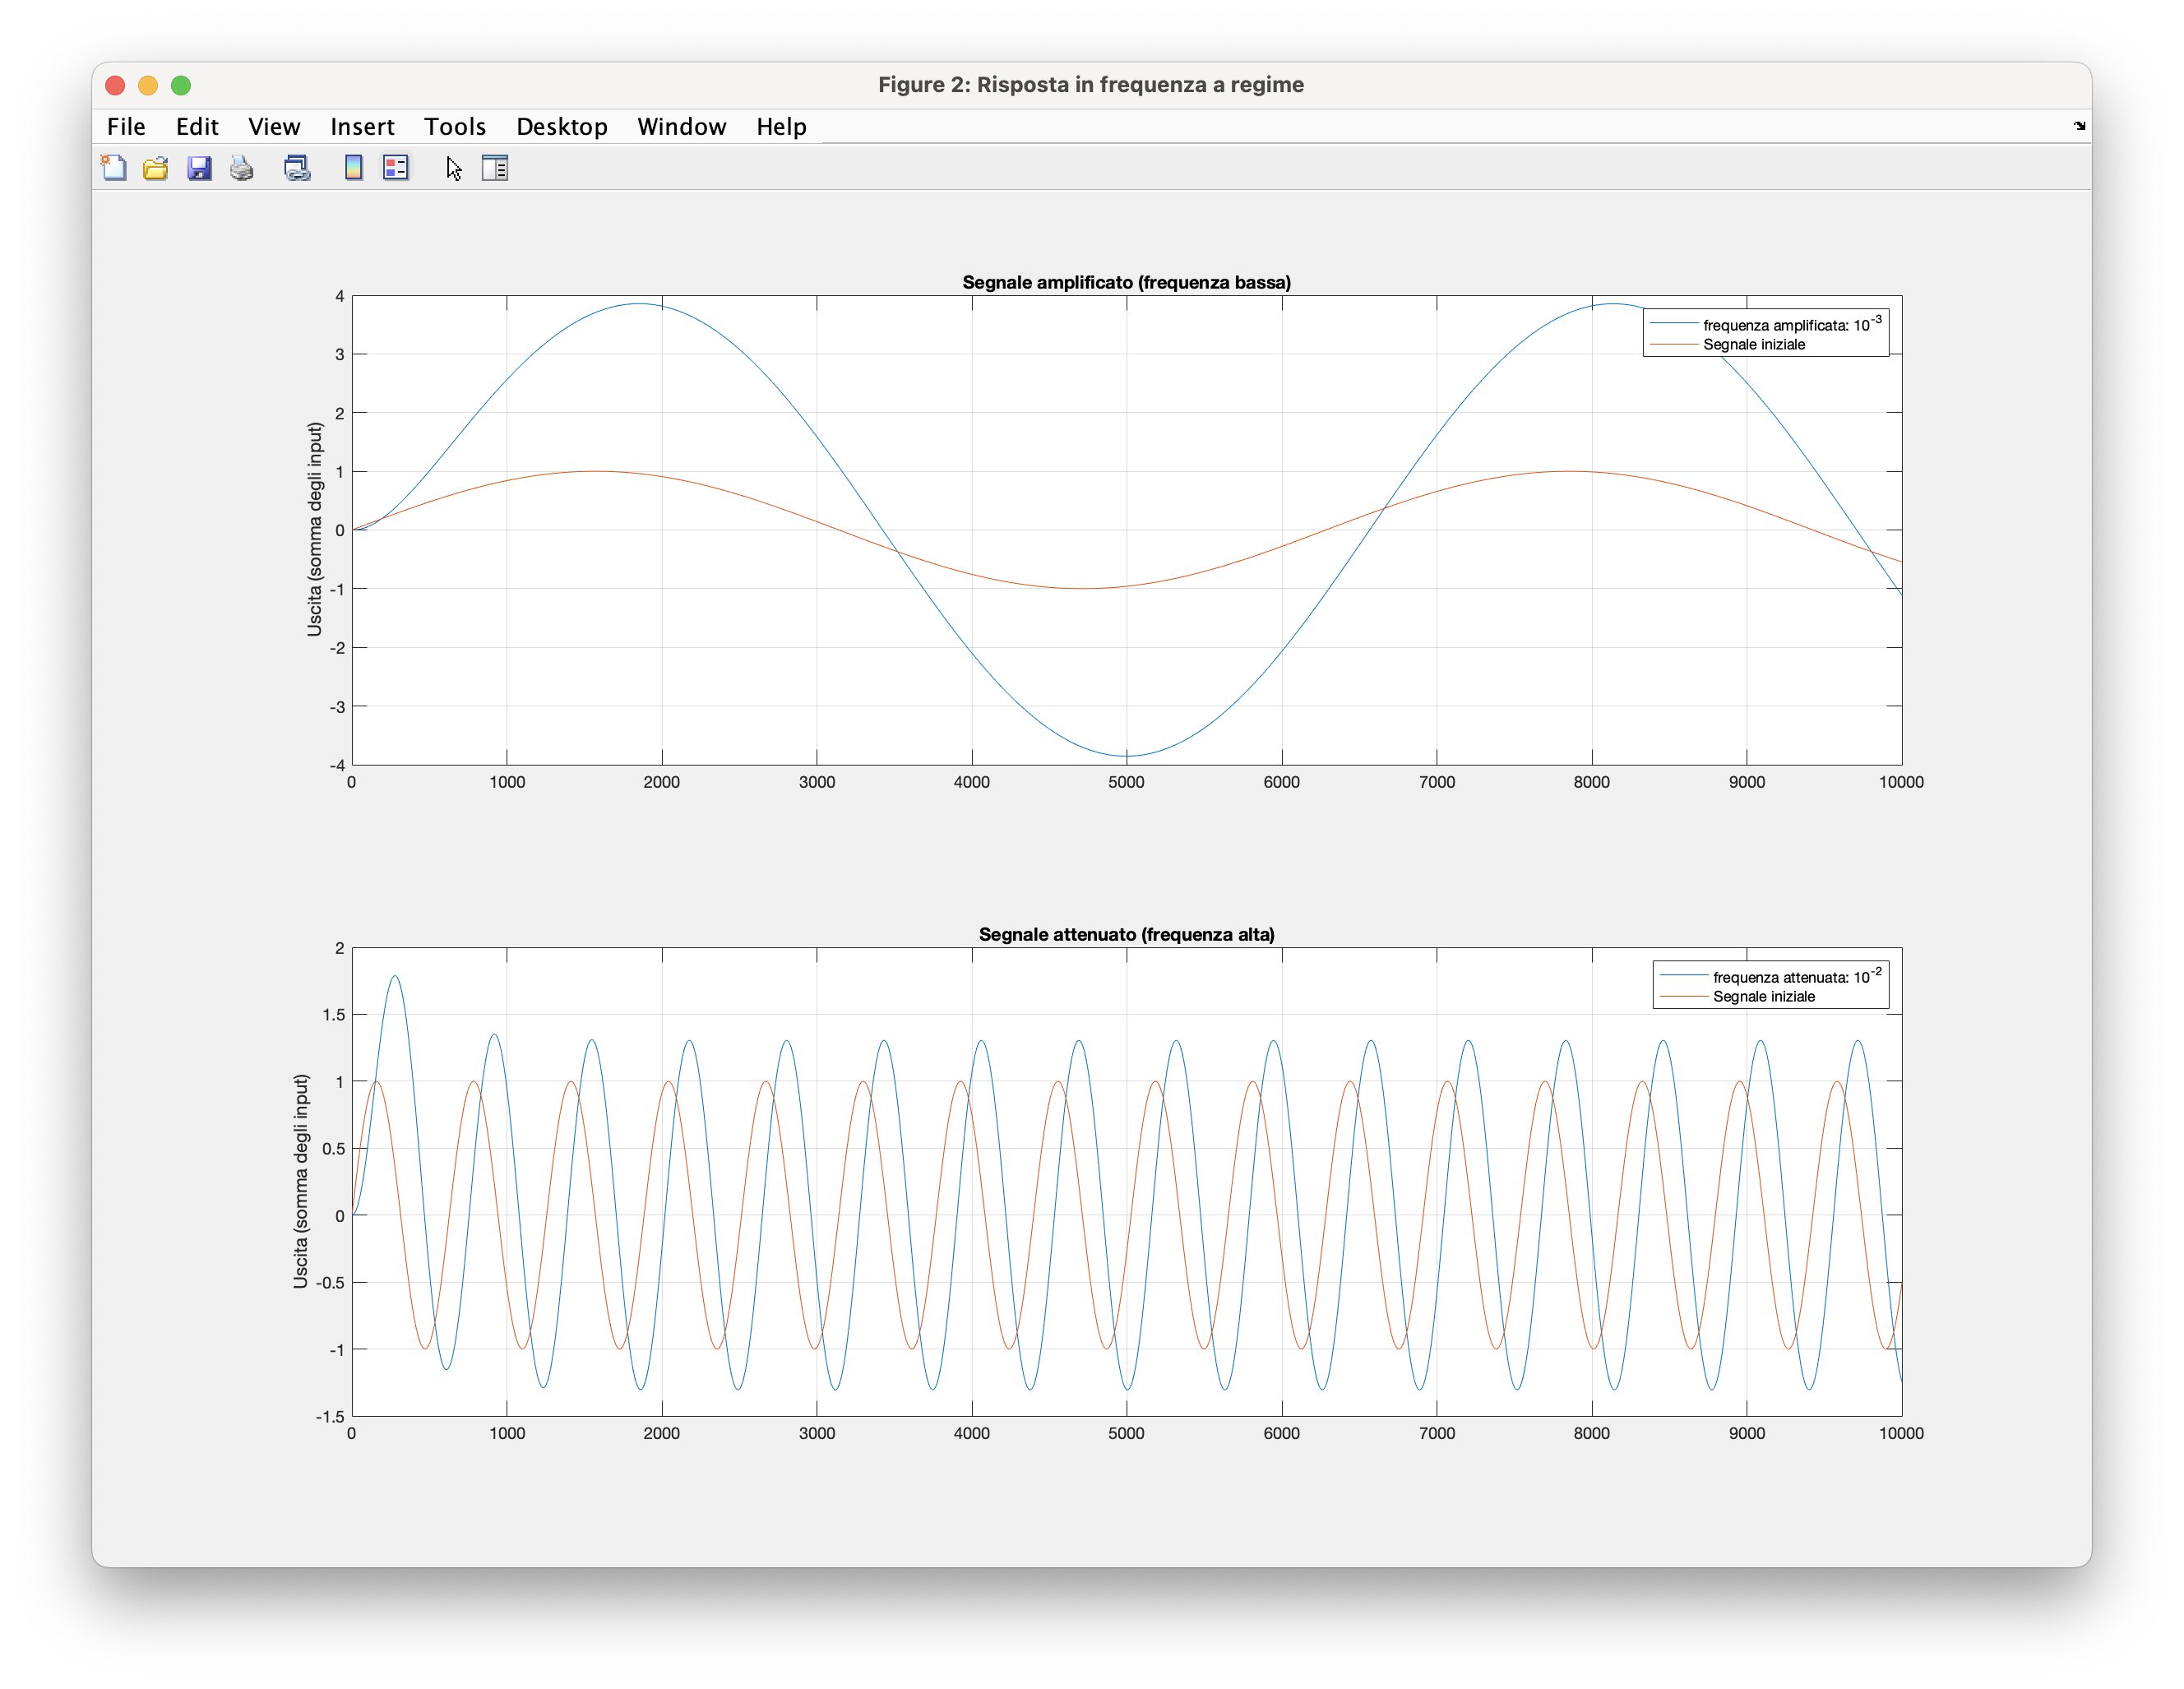
\includegraphics{/Users/follen/Desktop/SistemiDinamici/TESINA/assets/image-20240107212750287.png}

In questo esempio possiamo vedere due tipi di output, che vengono
calcolati a seconda dell\textquotesingle input. In blu osserviamo
l\textquotesingle output, mentre l\textquotesingle input è rappresentato
in arancione.

Nel primo caso, è stata scelta una frequenza tale che, a seconda delle
specifiche del sistema, porta l\textquotesingle output ad essere
\textbf{amplificato}; infatti possiamo osservare come il valore di
uscita (bisogna sempre tenere presente che l\textquotesingle output è la
somma di 3 contributi, visto che il sistema accetta 3 input) ha
un\textquotesingle ampiezza maggiore rispetto al segnale di entrata.

Nel secondo caso, è stata scelta una frequenza \textbf{più alta}, in
modo che l\textquotesingle output venisse \textbf{attenuato}.
Continuiamo ad osservare un\textquotesingle ampiezza finale maggiore
rispetto a quella del segnale di ingresso per il semplice motivo che il
segnale di output è la somma di 3 contributi.

L\textquotesingle intervallo di frequenze (banda) scelto è lo stesso per
entrambi i segnali, proprio per evidenziare le differenze di frequenza e
di fase.

\hypertarget{richieste}{%
\subsection{Richieste}\label{richieste}}

La prova orale consiste nella presentazione di un esempio simulato in
Matlab/Simulink e due domande dall'elenco allegato.

Un modello di traccia per la presentazione del modello da simulare (lo
studente deve portare con sé il codice oppure un portatile per mostrare
la simulazione) è il seguente:

\begin{itemize}
\item
  \textbf{Primo lucido}: disegno del sistema (si può scegliere tra
  quelli fatti a lezione eventualmente introducendo piccole varianti o
  un altro modello a scelta), equazioni, modello nello spazio di stato,
  funzione di trasferimento
\item
  \textbf{Secondo lucido}: parametri, risposta impulsiva con singoli
  modi (espressione analitica e rappresentazione grafica)
\item
  \textbf{Terzo lucido}: diagrammi di Bode e risposta a sinusoide/i
\item
  \textbf{Quarto lucido}: risposta nel tempo a diverse condizioni
  (\emph{ingressi}, \emph{parametri})
\end{itemize}

\end{document}
